\documentclass[12pt,a4paper]{article}
		\usepackage{amsmath}
		\usepackage{amsfonts}
		\usepackage{amssymb}
		\usepackage{pgf,tikz}
		\usepackage{mathrsfs}
		\usepackage{adjustbox}
		\usepackage{tabularx}
		\usepackage{multicol}
		\usepackage{etex}
		\usepackage{circuitikz}
		\usetikzlibrary {circuits.ee.IEC}
		\usepackage{pgf}
		\usepackage{bm}
		\usepackage{pstricks}
		\let\clipbox\relax
		\usetikzlibrary{arrows}
		\usepackage{lastpage}
		\usepackage{setspace}
		\usepackage{enumitem}
		\usepackage{graphicx} %table
		\usepackage{diagbox}
		\usepackage[left=0.75cm,right=0.75cm,top=0.5cm,bottom=0.75cm,includehead,includefoot]{geometry}
		\usepackage{xcolor}
		\usepackage{polyglossia}
		\usepackage{graphicx}
		\usepackage[most]{tcolorbox}
		\usepackage{titlesec}
		\usepackage{fancyhdr} % Mise en page, en-tête et pied de page
		\usepackage[a4,frame,center]{crop}
		\setdefaultlanguage[calendar=gregorian,numerals=maghrib]{arabic}
		\setotherlanguage{french}
		\newfontfamily\arabicfont[Script=Arabic,Scale=1]{Amiri}
		\newfontfamily\arabicfontsf[Script=Arabic,Scale=1]{Amiri}
		\newtcbtheorem[auto counter]{exercice}%
		{\textbf{تمرين}}{enhanced jigsaw,breakable,fonttitle=\bfseries\upshape,before skip=1mm,after skip=1mm,/tcb/bottom= 1 mm ,/tcb/top= 1 mm ,
			arc=0mm, colback=white!5!white,colframe=black!50!black}{theorem}
			%Solution ==================================================
		\newtcbtheorem[]{solution}%
		{\textbf{حل التمرين}}{enhanced jigsaw,breakable,/tcb/top=4mm,before skip=1mm,after skip=1mm,
		attach boxed title to top center={xshift=0cm,yshift=-3.7mm},
		fonttitle=\bfseries,varwidth boxed title=0.7\linewidth,
		colbacktitle=white!45!white,coltitle=white!10!black,colframe=white!50!black,
		interior style={top color=white!10!white,bottom color=white!10!white},
		boxed title style={boxrule=0.5mm,
		frame code={ \path[tcb fill frame] ([xshift=-4mm]frame.west)
		-- (frame.north west) -- (frame.north east) -- ([xshift=4mm]frame.east)
		-- (frame.south east) -- (frame.south west) -- cycle; },
		interior code={ \path[tcb fill interior] ([xshift=-2mm]interior.west)
		-- (interior.north west) -- (interior.north east)
		-- ([xshift=2mm]interior.east) -- (interior.south east) -- (interior.south west)
		-- cycle;} }
		,arc=0mm, colback=white!5!white,colframe=blue!50!white}{theorem}
		%============================================================
		\setlength{\columnseprule}{1pt}
		\def\columnseprulecolor{\color{blue}}
		\titlespacing{\section}{0pt}{0pt}{0pt}
		\pagestyle{fancy}
		\cfoot{\thepage}
		%\rfoot{}
		\definecolor{color1}{RGB}{0,0,0}
		\newcommand*\circled[1]{\tikz[baseline=(char.base)]{%
        \node[shape=circle,left color=color1!60!black,right color=color1!60!black,
		middle color=color1!80!black,draw,inner sep=1pt] (char) {#1};}}
		%==============================
		\newcommand*\rectled[1]{\tikz[baseline=(char.base)]{%
        \node[shape=rectangle,left color=color1!60!black,right color=color1!60!black,
		middle color=color1!80!black,draw,inner sep=1pt] (char) {#1};}}
		\lfoot{السنة الدراسية : 
  jjhhh }
\lhead{مادة : الفيزياء والكيمياء\\الأستاذ :  tggg  }
\rhead{الثانوية التأهيلية  : jjjjj \\المستوى الدراسي  :  kkkkk }
\rfoot{التجاذب الكوني}
\lfoot{kkkkk }
 \chead{\centering سلسلة تمارين\\ 
التجاذب الكوني}
\begin{document}
  
  %Exercice 7
\textbf{\begin{exercice}{}/
					إعط رتبة قدر الأعداد التالية :\\
					\begin{minipage}[c]{0.5\linewidth}
					\vspace{-0.3cm}
					\indent
					\textfrench{
						\begin{itemize}
							\item $\bm{ n_1=94= }\dotfill$
							\item $\bm{ n_2=0.0018= }\dotfill$
							\item $\bm{n_3=3.10^{2}= }\dotfill$
						\end{itemize}}
					\end{minipage}
					\begin{minipage}[c]{0.5\linewidth}
					\vspace{-0.3cm}
					\indent
					\textfrench{
						\begin{itemize}
							\item $\bm{n_4=8,7.10^{-3}=}\dotfill$
							\item $\bm{ n_5=7= }\dotfill$
							\item $\bm{ n_6=0= }\dotfill$
						\end{itemize}}
					\end{minipage}
					\end{exercice}}%=== source ===%
  %Exercice 4
\textbf{\begin{exercice}{}/
					\begin{flushright}
					نعتبر الأبعاد التالية :\\	
\begin{minipage}[c]{0.49\linewidth}
\indent
\vspace{-0.1cm}
					\begin{itemize}
					\item المسافة بین الأرض والقمر
					\hrulefill
					$\bm{A = 380\ 000\ km}$
					\item شعاع ذرة الھیدروجین
					\hrulefill
					$\bm{B=1,05.10^{-10}\ m}$
					\item ارتفاع جبل توبقال
					\hrulefill
					$\bm{C=4165\ m}$
					\item قطر جزیئة
					\hrulefill
					$\bm{D=2\ nm}$
					\item شعاع الأرض
					\hrulefill
					$\bm{E=6\ 400\ km}$ 
					\item قامة إنسان
					\hrulefill
					$\bm{F=170\ cm}$
					\end{itemize}
\end{minipage}
\begin{minipage}[c]{0.49\linewidth}	
\indent
\vspace{-0.1cm}	
\begin{itemize} 			
					\item المسافة بین الأرض و الشمس
					\hrulefill
					$\bm{G=150.10^{6}\ km}$
					\item شعاع نواة ذرة الھیدروجین
					\hrulefill
					$\bm{H=10^{-15}\ m }$
					\item قطر مجرتنا
					\hrulefill
					$\bm{I=9,5.10^{17}\ km }$ 
					\item قطر خلیة
					\hrulefill
					$\bm{J=10\ \mu m }$
					\item شعاع الشمس
					\hrulefill
					$\bm{K=700\ 000\ km }$ 
					\item القطر التقریبي للكون
					\hrulefill
					$\bm{L=12.10^{22}\ km }$ 
					\end{itemize}
\end{minipage}
					\begin{enumerate}[leftmargin=*,label=\protect\circled{\color{white}\textbf{\arabic*}}]
					\item حول الى الوحدة العالمية إن كان ممكنا.
					\item أكتب هذه الأبعاد كتابة علمية.
					\item استنتج رتب القدر.
					\item مثل  هذه المسافات على محور سلم المسافات.
					\end{enumerate}
					\end{flushright}
					\end{exercice}}%=== source ===%
  %Exercice 2
\textbf{\begin{exercice}{}/
					\begin{minipage}[c]{0.65\linewidth}
					\indent
					\vspace{-0.7cm}
					\begin{enumerate}[label=\protect\circled{\color{white}\textbf{\arabic*}}]
					\item إعط مميزات القوة التي تسلطها الأرض على القمر.
					\item إستنتج شدة القوة التي يسلطها القمر على الأرض.
					\item  مثل القوتين على الشكل
			باستعمال سلم مناسب.
					\\المعطيات:
					\begin{itemize}
					\item كتلة الأرض $\bm{M_T=5,97.10^{24}\ kg}\hrulefill$
					\item كتلة القمر
					$\bm{M_L=7,35.10^{22}\ kg}\hrulefill$
					\item المسافة بين الأرض والقمر
					$\bm{d=3,84.10^8\ m}\hrulefill$
					\item	ثابتة التجاذب الكوني 
					$\bm{G=6,67.10^{-11}\ N.m^2.kg^{-1}}\hrulefill$
					\end{itemize}
					\end{enumerate}
					\end{minipage}
					\begin{minipage}[c]{0.34\linewidth}
\definecolor{cffffff}{RGB}{255,255,255}
\definecolor{cffaf00}{RGB}{255,175,0}
\definecolor{c5260e5}{RGB}{82,96,229}
\definecolor{c288029}{RGB}{40,128,41}
\definecolor{c3498db}{RGB}{52,152,219}
\begin{flushleft}
\begin{adjustbox}{width=\linewidth}
\fbox{\begin{tikzpicture}[y=0.80pt, x=0.80pt, yscale=-1.000000, xscale=1.000000, inner sep=0pt, outer sep=0pt]
\begin{scope}[shift={(-311.0,-268.0)}]
  \path[shift={(312.0,269.0)},draw=black,fill=cffffff] (0.0000,0.0000) --
    (307.0000,0.0000) -- (307.0000,288.0000) -- (0.0000,288.0000) --
    (0.0000,0.0000) -- cycle;
  \path[shift={(522.51,310.5)},draw=black,fill=cffaf00] (0.0000,38.8000) ..
    controls (0.0000,17.3000) and (17.3000,0.0000) .. (38.8000,0.0000) .. controls
    (60.2000,0.0000) and (77.5000,17.3000) .. (77.5000,38.8000) .. controls
    (77.5000,60.2000) and (60.2000,77.5000) .. (38.8000,77.5000) .. controls
    (17.3000,77.5000) and (0.0000,60.2000) .. (0.0000,38.8000) -- cycle;
  \begin{scope}[shift={(321.0,402.0)}]
      \path[cm={{-1.0,0.0,0.0,1.0,(155.2,0.0)}},fill=c5260e5] (0.0000,74.0000) ..
        controls (0.0000,33.1000) and (34.7000,0.0000) .. (77.6000,0.0000) .. controls
        (120.5000,0.0000) and (155.2000,33.1000) .. (155.2000,74.0000) .. controls
        (155.2000,114.8000) and (120.5000,148.0000) .. (77.6000,148.0000) .. controls
        (34.7000,148.0000) and (0.0000,114.8000) .. (0.0000,74.0000) -- cycle;
    \path[shift={(39.29,30.75)},fill=c288029] (0.7000,10.9000) .. controls
      (3.7000,10.9000) and (4.3000,10.1000) .. (4.3000,9.5000) .. controls
      (4.3000,8.9000) and (4.3000,7.9000) .. (5.0000,7.3000) .. controls
      (5.6000,6.7000) and (6.2000,6.4000) .. (6.2000,6.4000) .. controls
      (6.2000,6.4000) and (6.8000,6.7000) .. (6.2000,8.1000) .. controls
      (5.6000,9.5000) and (5.0000,10.1000) .. (5.0000,10.1000) -- (7.0000,10.5000)
      .. controls (7.0000,10.5000) and (8.2000,9.8000) .. (8.2000,10.1000) ..
      controls (8.2000,10.4000) and (9.5000,9.5000) .. (10.0000,9.5000) .. controls
      (10.4000,9.5000) and (11.1000,8.1000) .. (11.1000,8.1000) .. controls
      (11.1000,8.1000) and (10.7000,7.7000) .. (11.1000,7.3000) .. controls
      (11.5000,6.9000) and (10.4000,5.9000) .. (10.4000,5.9000) .. controls
      (10.4000,5.9000) and (9.7000,5.1000) .. (9.2000,4.0000) .. controls
      (8.6000,3.0000) and (9.0000,4.0000) .. (8.6000,3.0000) .. controls
      (8.2000,2.0000) and (6.8000,0.3000) .. (7.2000,0.3000) .. controls
      (7.6000,0.3000) and (6.8000,0.3000) .. (6.8000,0.3000) .. controls
      (6.8000,0.3000) and (6.1000,-0.4000) .. (5.3000,0.2000) .. controls
      (4.6000,0.8000) and (4.3000,0.6000) .. (4.3000,1.7000) .. controls
      (4.3000,2.8000) and (4.3000,3.0000) .. (4.3000,3.7000) .. controls
      (4.3000,4.5000) and (3.2000,4.8000) .. (3.0000,5.4000) .. controls
      (2.8000,5.9000) and (1.7000,6.4000) .. (1.2000,6.4000) .. controls
      (0.7000,6.4000) and (-0.5000,6.5000) .. (0.2000,7.3000) .. controls
      (1.0000,8.1000) and (1.7000,8.1000) .. (2.0000,8.1000) .. controls
      (2.3000,8.1000) and (0.7000,9.9000) .. (0.7000,10.4000) .. controls
      (0.7000,10.9000) and (0.7000,11.5000) .. (0.7000,10.9000) -- cycle;
    \path[shift={(36.2,0.87)},fill=c288029] (55.2000,59.6000) -- (55.3000,60.9000)
      .. controls (55.3000,60.9000) and (56.1000,62.2000) .. (56.5000,62.3000) ..
      controls (56.8000,62.5000) and (58.7000,63.3000) .. (58.7000,63.9000) ..
      controls (58.7000,64.5000) and (59.8000,65.7000) .. (59.8000,65.7000) --
      (61.1000,66.9000) .. controls (61.1000,66.9000) and (62.7000,69.2000) ..
      (62.7000,70.1000) .. controls (62.7000,71.0000) and (63.7000,71.0000) ..
      (63.5000,70.9000) .. controls (63.5000,70.9000) and (64.9000,71.3000) ..
      (64.9000,71.8000) .. controls (64.9000,72.3000) and (66.0000,74.9000) ..
      (67.6000,74.9000) .. controls (69.2000,74.9000) and (70.1000,76.6000) ..
      (70.1000,76.6000) .. controls (70.1000,76.6000) and (71.8000,77.5000) ..
      (71.8000,77.5000) .. controls (71.8000,77.5000) and (70.7000,80.4000) ..
      (74.6000,78.6000) .. controls (76.1000,78.0000) and (77.0000,76.6000) ..
      (77.0000,76.6000) -- (80.0000,75.8000) .. controls (80.0000,75.8000) and
      (80.6000,76.5000) .. (80.0000,78.6000) .. controls (79.3000,80.8000) and
      (79.5000,83.2000) .. (78.9000,83.9000) .. controls (78.2000,84.6000) and
      (77.3000,85.1000) .. (76.4000,87.2000) .. controls (75.4000,89.2000) and
      (73.9000,90.9000) .. (73.1000,92.1000) .. controls (72.3000,93.4000) and
      (69.8000,96.2000) .. (69.8000,98.3000) .. controls (69.8000,100.5000) and
      (69.3000,101.6000) .. (70.6000,102.8000) .. controls (71.8000,104.1000) and
      (71.8000,104.5000) .. (71.8000,106.7000) .. controls (71.8000,108.9000) and
      (72.2000,110.1000) .. (70.1000,111.4000) .. controls (68.1000,112.6000) and
      (67.0000,114.3000) .. (67.0000,115.0000) .. controls (67.0000,115.6000) and
      (67.7000,118.2000) .. (65.7000,121.3000) .. controls (64.8000,122.7000) and
      (65.7000,121.3000) .. (65.7000,121.3000) .. controls (65.7000,121.3000) and
      (65.7000,122.9000) .. (63.7000,126.6000) .. controls (61.6000,130.3000) and
      (60.4000,130.0000) .. (58.7000,130.5000) .. controls (56.9000,130.9000) and
      (55.7000,132.4000) .. (55.7000,132.4000) .. controls (55.7000,132.4000) and
      (55.1000,132.6000) .. (53.2000,129.2000) .. controls (51.3000,125.8000) and
      (51.8000,129.4000) .. (50.8000,128.0000) .. controls (49.9000,126.6000) and
      (48.8000,124.1000) .. (48.6000,123.8000) .. controls (48.5000,123.5000) and
      (48.2000,123.2000) .. (47.4000,121.8000) .. controls (46.6000,120.4000) and
      (46.1000,120.5000) .. (45.3000,119.7000) .. controls (44.4000,118.8000) and
      (43.2000,115.3000) .. (43.8000,111.7000) .. controls (43.9000,110.6000) and
      (42.4000,108.0000) .. (40.9000,106.3000) .. controls (39.5000,104.5000) and
      (38.0000,103.5000) .. (36.6000,102.8000) .. controls (35.1000,102.2000) and
      (35.0000,99.7000) .. (34.8000,98.8000) .. controls (34.7000,97.9000) and
      (32.8000,94.5000) .. (31.3000,95.3000) .. controls (29.8000,96.1000) and
      (29.4000,96.6000) .. (28.5000,94.8000) .. controls (27.6000,93.1000) and
      (22.5000,97.3000) .. (21.4000,98.3000) .. controls (20.3000,99.4000) and
      (19.0000,97.7000) .. (15.4000,99.3000) .. controls (11.8000,100.8000) and
      (13.2000,99.3000) .. (9.8000,98.3000) .. controls (6.3000,97.4000) and
      (8.0000,95.5000) .. (4.1000,93.8000) .. controls (0.2000,92.1000) and
      (1.6000,91.2000) .. (1.6000,90.3000) .. controls (1.6000,89.3000) and
      (1.9000,85.6000) .. (0.7000,83.4000) .. controls (-0.6000,81.3000) and
      (0.0000,79.2000) .. (0.9000,76.6000) .. controls (2.1000,74.0000) and
      (3.0000,72.0000) .. (4.4000,71.0000) .. controls (5.8000,70.1000) and
      (4.0000,69.5000) .. (4.4000,67.9000) .. controls (4.9000,66.4000) and
      (8.0000,64.2000) .. (8.0000,61.9000) .. controls (8.0000,59.5000) and
      (8.7000,62.8000) .. (10.5000,61.9000) .. controls (12.4000,60.9000) and
      (14.6000,60.2000) .. (16.0000,58.8000) .. controls (17.4000,57.4000) and
      (18.9000,57.0000) .. (20.6000,56.7000) .. controls (22.3000,56.4000) and
      (24.6000,55.5000) .. (25.6000,55.5000) .. controls (26.5000,55.5000) and
      (26.7000,57.2000) .. (26.8000,57.5000) .. controls (27.0000,57.8000) and
      (25.2000,58.9000) .. (26.8000,59.4000) .. controls (28.5000,59.8000) and
      (31.2000,60.5000) .. (32.2000,60.5000) .. controls (33.1000,60.5000) and
      (38.2000,62.8000) .. (38.8000,60.5000) .. controls (39.4000,57.8000) and
      (40.9000,57.8000) .. (42.8000,58.3000) .. controls (44.7000,58.8000) and
      (45.8000,59.1000) .. (47.4000,58.3000) .. controls (48.9000,57.5000) and
      (51.1000,56.7000) .. (53.8000,56.7000) .. controls (56.5000,56.7000) and
      (55.7000,50.5000) .. (55.7000,49.6000) .. controls (55.7000,48.7000) and
      (54.1000,48.4000) .. (53.2000,49.3000) .. controls (52.3000,50.2000) and
      (52.7000,51.1000) .. (50.8000,50.4000) .. controls (48.9000,49.6000) and
      (48.5000,52.5000) .. (45.6000,51.0000) .. controls (42.8000,49.5000) and
      (44.7000,48.2000) .. (42.3000,47.3000) .. controls (39.8000,46.5000) and
      (38.0000,49.0000) .. (38.8000,49.3000) .. controls (39.5000,49.6000) and
      (43.1000,54.1000) .. (39.5000,52.2000) .. controls (35.9000,50.4000) and
      (37.3000,48.0000) .. (36.1000,48.8000) .. controls (34.8000,49.6000) and
      (35.9000,48.1000) .. (34.2000,47.0000) .. controls (32.0000,45.4000) and
      (29.0000,45.7000) .. (29.0000,44.6000) .. controls (29.0000,43.4000) and
      (27.3000,42.3000) .. (26.8000,43.2000) .. controls (26.4000,44.2000) and
      (26.6000,45.8000) .. (29.0000,46.7000) .. controls (31.3000,47.7000) and
      (32.9000,48.5000) .. (33.3000,48.9000) .. controls (33.7000,49.2000) and
      (33.7000,49.6000) .. (32.6000,49.6000) .. controls (31.5000,49.6000) and
      (34.0000,51.1000) .. (32.8000,52.2000) .. controls (31.6000,53.4000) and
      (30.2000,53.7000) .. (30.8000,53.6000) .. controls (31.3000,53.6000) and
      (34.1000,56.4000) .. (29.0000,54.6000) .. controls (23.9000,52.9000) and
      (28.8000,53.6000) .. (30.1000,52.9000) .. controls (31.3000,52.2000) and
      (35.0000,50.2000) .. (27.8000,49.6000) .. controls (20.6000,49.0000) and
      (25.6000,49.1000) .. (24.4000,47.3000) .. controls (23.2000,45.6000) and
      (21.4000,47.7000) .. (21.4000,48.0000) .. controls (21.4000,48.4000) and
      (19.0000,48.8000) .. (18.1000,48.8000) .. controls (17.1000,48.8000) and
      (17.5000,52.2000) .. (15.4000,53.6000) .. controls (13.3000,55.1000) and
      (14.6000,56.3000) .. (14.1000,57.5000) .. controls (13.7000,58.8000) and
      (11.8000,61.2000) .. (6.9000,59.4000) .. controls (2.1000,57.5000) and
      (6.0000,57.8000) .. (4.9000,55.5000) .. controls (3.5000,52.4000) and
      (7.8000,50.0000) .. (7.4000,50.4000) .. controls (7.4000,50.4000) and
      (12.9000,48.2000) .. (12.0000,46.7000) .. controls (11.0000,45.2000) and
      (11.0000,44.9000) .. (9.0000,44.9000) .. controls (6.9000,44.9000) and
      (7.8000,42.8000) .. (10.5000,42.3000) .. controls (13.3000,41.8000) and
      (13.6000,39.1000) .. (15.7000,37.5000) .. controls (17.8000,35.9000) and
      (16.0000,35.5000) .. (18.9000,34.5000) .. controls (21.7000,33.6000) and
      (18.5000,29.9000) .. (21.8000,29.1000) .. controls (23.4000,28.7000) and
      (23.7000,32.2000) .. (24.4000,28.6000) .. controls (24.7000,27.3000) and
      (22.6000,25.8000) .. (22.2000,25.5000) .. controls (21.8000,25.1000) and
      (20.1000,29.7000) .. (18.9000,28.5000) .. controls (17.6000,27.3000) and
      (16.7000,26.6000) .. (17.7000,24.9000) .. controls (18.4000,23.7000) and
      (23.1000,19.2000) .. (23.6000,17.5000) .. controls (24.0000,15.8000) and
      (24.8000,14.4000) .. (27.8000,12.6000) .. controls (30.8000,10.9000) and
      (36.6000,8.0000) .. (38.8000,9.1000) .. controls (40.9000,10.2000) and
      (42.5000,11.9000) .. (44.5000,8.7000) .. controls (46.4000,5.5000) and
      (46.7000,6.9000) .. (46.7000,6.9000) .. controls (44.1000,5.2000) and
      (42.6000,3.8000) .. (42.0000,2.6000) .. controls (41.5000,1.3000) and
      (44.2000,0.9000) .. (44.1000,2.6000) .. controls (43.7000,6.7000) and
      (53.2000,5.9000) .. (53.2000,5.9000) .. controls (53.2000,5.9000) and
      (50.4000,5.4000) .. (50.0000,4.3000) .. controls (49.6000,3.3000) and
      (51.9000,3.6000) .. (53.8000,4.0000) .. controls (55.7000,4.3000) and
      (54.8000,2.9000) .. (53.2000,2.6000) .. controls (51.5000,2.2000) and
      (52.5000,0.7000) .. (52.2000,1.0000) .. controls (51.9000,1.3000) and
      (50.3000,0.9000) .. (50.3000,0.9000) .. controls (49.3000,0.0000) and
      (68.4000,0.4000) .. (87.8000,13.7000) .. controls (107.2000,27.1000) and
      (114.0000,47.1000) .. (116.5000,55.5000) .. controls (116.5000,55.5000) and
      (116.5000,55.5000) .. (116.5000,55.5000) .. controls (116.5000,55.5000) and
      (115.6000,54.8000) .. (115.7000,55.5000) .. controls (115.8000,56.2000) and
      (117.9000,64.5000) .. (117.9000,66.2000) .. controls (117.9000,67.6000) and
      (117.4000,69.8000) .. (117.4000,70.4000) .. controls (117.4000,71.0000) and
      (117.2000,67.5000) .. (115.7000,66.2000) .. controls (114.2000,64.6000) and
      (115.7000,70.4000) .. (115.7000,70.4000) .. controls (115.7000,70.4000) and
      (117.9000,77.5000) .. (117.9000,78.8000) .. controls (117.9000,80.0000) and
      (117.4000,84.2000) .. (117.4000,81.4000) .. controls (117.4000,81.4000) and
      (117.3000,89.2000) .. (116.5000,89.3000) .. controls (115.7000,89.5000) and
      (117.1000,81.5000) .. (114.9000,76.6000) .. controls (114.0000,74.4000) and
      (116.5000,77.5000) .. (116.5000,76.6000) .. controls (116.5000,75.7000) and
      (115.0000,70.4000) .. (114.9000,69.6000) .. controls (114.7000,66.2000) and
      (115.2000,63.7000) .. (114.6000,62.7000) .. controls (113.9000,61.6000) and
      (113.3000,62.0000) .. (111.9000,58.8000) .. controls (110.7000,56.4000) and
      (109.4000,55.3000) .. (109.9000,55.5000) .. controls (109.9000,55.5000) and
      (108.2000,53.3000) .. (107.6000,57.0000) .. controls (107.1000,60.0000) and
      (106.5000,63.4000) .. (105.5000,65.1000) .. controls (103.8000,68.3000) and
      (106.3000,73.4000) .. (104.9000,74.3000) .. controls (103.0000,75.4000) and
      (103.2000,71.8000) .. (102.2000,70.4000) .. controls (102.2000,70.4000) and
      (98.9000,63.7000) .. (98.9000,62.5000) .. controls (98.9000,61.2000) and
      (98.7000,60.5000) .. (98.1000,60.5000) .. controls (97.3000,60.5000) and
      (96.5000,60.8000) .. (95.2000,59.8000) .. controls (91.8000,57.4000) and
      (93.1000,58.8000) .. (93.3000,58.5000) .. controls (93.4000,58.2000) and
      (91.6000,58.3000) .. (91.6000,56.7000) .. controls (91.6000,55.2000) and
      (86.4000,58.9000) .. (84.0000,57.8000) .. controls (81.7000,56.7000) and
      (82.2000,56.1000) .. (81.5000,56.1000) .. controls (80.9000,56.1000) and
      (80.2000,56.2000) .. (79.7000,56.7000) .. controls (79.1000,57.3000) and
      (77.8000,57.4000) .. (76.5000,56.7000) .. controls (75.3000,56.1000) and
      (73.0000,52.6000) .. (71.5000,54.9000) .. controls (71.5000,54.9000) and
      (72.3000,57.5000) .. (74.6000,58.6000) .. controls (75.8000,59.1000) and
      (79.2000,60.5000) .. (81.5000,58.4000) .. controls (82.9000,57.1000) and
      (81.4000,59.2000) .. (84.0000,59.8000) .. controls (86.7000,60.5000) and
      (85.9000,65.1000) .. (82.8000,68.1000) .. controls (79.7000,71.0000) and
      (79.8000,72.4000) .. (77.9000,73.3000) .. controls (76.2000,74.2000) and
      (74.2000,75.4000) .. (73.4000,76.1000) .. controls (72.6000,76.9000) and
      (71.4000,77.7000) .. (70.3000,73.0000) .. controls (69.2000,68.4000) and
      (69.7000,69.7000) .. (67.1000,69.2000) .. controls (64.5000,68.6000) and
      (64.0000,65.7000) .. (62.8000,64.9000) .. controls (61.6000,64.0000) and
      (57.2000,59.9000) .. (57.2000,59.9000) -- (55.2000,59.6000) -- cycle;
    \path[shift={(17.97,1.78)}] (42.0000,0.6000) .. controls (42.0000,0.6000) and
      (35.8000,2.7000) .. (34.8000,3.4000) .. controls (33.7000,4.0000) and
      (33.8000,5.1000) .. (31.9000,5.1000) .. controls (30.1000,5.1000) and
      (30.1000,5.4000) .. (29.4000,6.5000) .. controls (28.8000,7.5000) and
      (28.0000,8.0000) .. (27.1000,8.3000) .. controls (26.1000,8.6000) and
      (25.6000,8.9000) .. (25.2000,9.7000) .. controls (24.8000,10.6000) and
      (22.7000,12.4000) .. (21.7000,12.4000) .. controls (20.8000,12.4000) and
      (20.6000,13.0000) .. (20.6000,13.5000) .. controls (20.6000,14.1000) and
      (20.8000,14.2000) .. (17.7000,16.3000) .. controls (14.7000,18.4000) and
      (13.3000,18.9000) .. (12.2000,19.7000) .. controls (9.5000,21.5000) and
      (9.7000,21.8000) .. (6.7000,24.0000) .. controls (3.2000,26.5000) and
      (2.0000,31.3000) .. (0.9000,32.4000) .. controls (-0.2000,33.5000) and
      (-0.4000,30.6000) .. (0.9000,27.7000) .. controls (2.0000,25.4000) and
      (6.0000,20.5000) .. (7.5000,19.0000) .. controls (9.0000,17.6000) and
      (16.8000,11.1000) .. (17.7000,10.2000) .. controls (18.6000,9.3000) and
      (34.4000,1.0000) .. (42.0000,0.3000) .. controls (49.5000,-0.5000) and
      (42.0000,0.6000) .. (42.0000,0.6000) -- cycle;
    \path[shift={(2.66,31.91)},fill=c288029] (8.8000,4.4000) .. controls
      (8.8000,4.4000) and (7.4000,7.0000) .. (6.5000,9.1000) .. controls
      (6.1000,10.0000) and (6.8000,12.9000) .. (6.0000,14.4000) .. controls
      (5.2000,16.0000) and (5.1000,17.1000) .. (5.1000,17.1000) .. controls
      (5.1000,17.1000) and (4.3000,19.8000) .. (4.3000,21.6000) .. controls
      (4.3000,23.3000) and (2.3000,24.0000) .. (2.3000,22.6000) .. controls
      (2.3000,21.2000) and (2.9000,18.8000) .. (3.4000,17.4000) .. controls
      (4.1000,15.8000) and (2.2000,20.0000) .. (2.2000,20.3000) -- (0.8000,26.3000)
      .. controls (0.3000,26.7000) and (0.0000,25.4000) .. (0.0000,25.4000) ..
      controls (0.0000,25.4000) and (1.7000,12.7000) .. (11.1000,0.0000) .. controls
      (11.4000,-0.4000) and (8.8000,4.4000) .. (8.8000,4.4000) -- cycle;
    \path[shift={(4.43,99.08)},fill=c288029] (0.0000,0.1000) .. controls
      (0.7000,0.1000) and (0.0000,0.1000) .. (2.0000,1.1000) .. controls
      (2.5000,1.4000) and (4.6000,3.8000) .. (5.0000,4.2000) .. controls
      (5.4000,4.6000) and (7.5000,5.4000) .. (11.1000,11.0000) .. controls
      (11.1000,11.0000) and (15.0000,12.0000) .. (15.6000,12.9000) .. controls
      (16.2000,13.9000) and (17.5000,12.5000) .. (18.4000,12.9000) .. controls
      (19.4000,13.4000) and (26.4000,14.3000) .. (26.4000,21.3000) .. controls
      (26.4000,21.3000) and (26.6000,23.6000) .. (29.2000,26.1000) .. controls
      (31.8000,28.7000) and (31.6000,30.8000) .. (31.6000,32.5000) .. controls
      (31.6000,34.2000) and (37.4000,38.7000) .. (41.4000,41.0000) .. controls
      (45.5000,43.4000) and (50.3000,45.6000) .. (50.6000,45.6000) .. controls
      (50.8000,45.5000) and (16.4000,38.4000) .. (0.0000,0.1000) .. controls
      (0.0000,-0.2000) and (0.0000,0.1000) .. (0.0000,0.1000) -- cycle;
    \path[shift={(110.88,104.97)},fill=c288029] (5.6000,0.0000) .. controls
      (5.6000,0.0000) and (7.5000,2.5000) .. (6.6000,2.9000) .. controls
      (5.6000,3.4000) and (5.6000,5.9000) .. (5.6000,4.3000) .. controls
      (5.6000,4.3000) and (5.5000,7.9000) .. (4.2000,10.1000) .. controls
      (2.9000,12.3000) and (4.4000,13.7000) .. (2.0000,14.1000) .. controls
      (-0.3000,14.6000) and (-0.0000,13.0000) .. (-0.0000,11.8000) .. controls
      (-0.0000,10.5000) and (1.4000,7.9000) .. (1.0000,6.9000) .. controls
      (0.6000,5.9000) and (1.1000,4.2000) .. (2.6000,3.6000) .. controls
      (4.2000,2.9000) and (4.6000,1.0000) .. (5.6000,0.0000) -- cycle;
  \end{scope}
  \path[cm={{-0.79,0.61,-0.61,-0.79,(562.0,350.0)}},draw=black,dash pattern=on
    2.00pt off 2.00pt,line width=2.400pt] (0.0000,0.0000) -- (208.2000,0.0000);
  \begin{scope}[shift={(524.01,278.5)}]
    \path (38,9.5) node[] (text29) {\Large \textbf{القمر}};
  \end{scope}
  \begin{scope}[shift={(360.61,368.0)}]
    \path (38,9.5) node[] (text29) {\Large \textbf{الأرض}};
  \end{scope}
  \path[shift={(556.23,347.47)},draw=black,fill=cffffff,line width=2.133pt]
    (0.0000,3.8000) .. controls (0.0000,1.7000) and (1.7000,0.0000) ..
    (3.8000,0.0000) .. controls (5.9000,0.0000) and (7.6000,1.7000) ..
    (7.6000,3.8000) .. controls (7.6000,5.9000) and (5.9000,7.6000) ..
    (3.8000,7.6000) .. controls (1.7000,7.6000) and (0.0000,5.9000) ..
    (0.0000,3.8000) -- cycle;
  \path[shift={(397.44,469.0)},draw=black,fill=cffffff,line width=2.133pt]
    (0.0000,3.8000) .. controls (0.0000,1.7000) and (1.7000,0.0000) ..
    (3.8000,0.0000) .. controls (5.9000,0.0000) and (7.6000,1.7000) ..
    (7.6000,3.8000) .. controls (7.6000,5.9000) and (5.9000,7.6000) ..
    (3.8000,7.6000) .. controls (1.7000,7.6000) and (0.0000,5.9000) ..
    (0.0000,3.8000) -- cycle;
\end{scope}
\end{tikzpicture}}
\end{adjustbox}
\end{flushleft}
					\end{minipage}
					\end{exercice}}%=== source ===%  
  %Exercice 3
\textbf{\begin{exercice}{}/
					كرتان مماثلتان ذات الكتلة 
					$\bm{m_A=m_B=100\ kg}$
					تفصل بينهما مسافة 
					$\bm{d=1m}$
					توجدان على سطح الأرض.
\begin{minipage}[c]{0.59\linewidth}
\indent					
					\begin{enumerate}[label=\protect\circled{\color{white}\textbf{\arabic*}}]
					\item أحسب شدة قوة التجاذب الكوني التي تسلطها الكرة على الأخرى.
					\item أحسب شدة قوة التجاذب الكوني التي تسلطها الأرض على إحدى الكرتين.
					\item  قارن بين هاتين الشدتين ماذا تستنتج؟
					\end{enumerate}
					\vspace{0.3cm}
\end{minipage}
					\begin{minipage}[c]{0.39\linewidth}
					\definecolor{cffffff}{RGB}{255,255,255}
\definecolor{cee7c31}{RGB}{238,124,49}
\definecolor{c3498db}{RGB}{52,152,219}
\begin{flushleft}
\begin{adjustbox}{width=\linewidth}
\fbox{
\begin{tikzpicture}[y=0.80pt, x=0.80pt, yscale=-1.000000, xscale=1.000000, inner sep=0pt, outer sep=0pt]
\begin{scope}[shift={(-334.0,-793.5)}]
  \path[shift={(335.0,798.0)},draw=black,fill=cffffff] (0.0000,0.0000) --
    (397.0000,0.0000) -- (397.0000,156.0000) -- (0.0000,156.0000) --
    (0.0000,0.0000) -- cycle;
  \path[shift={(348.61,833.0)},draw=black,fill=cffffff,line width=1.600pt]
    (0.0000,50.0000) .. controls (0.0000,22.4000) and (22.4000,0.0000) ..
    (50.0000,0.0000) .. controls (77.6000,0.0000) and (100.0000,22.4000) ..
    (100.0000,50.0000) .. controls (100.0000,77.6000) and (77.6000,100.0000) ..
    (50.0000,100.0000) .. controls (22.4000,100.0000) and (0.0000,77.6000) ..
    (0.0000,50.0000) -- cycle;
  \begin{scope}[shift={(350.0,933.0)}]
    \path[draw=cffffff,fill=cee7c31,line width=1.600pt] (0.0000,0.0000) --
      (363.0000,0.0000) -- (363.0000,12.0000) -- (0.0000,12.0000) -- (0.0000,0.0000)
      -- cycle;
    \path[shift={(2.14,0)},draw=black,line width=1.600pt] (0.0000,0.0000) --
      (360.9000,0.0000);
  \end{scope}
  \path[shift={(616.0,833.0)},draw=black,fill=cffffff,line width=1.600pt]
    (0.0000,50.0000) .. controls (0.0000,22.4000) and (22.4000,0.0000) ..
    (50.0000,0.0000) .. controls (77.6000,0.0000) and (100.0000,22.4000) ..
    (100.0000,50.0000) .. controls (100.0000,77.6000) and (77.6000,100.0000) ..
    (50.0000,100.0000) .. controls (22.4000,100.0000) and (0.0000,77.6000) ..
    (0.0000,50.0000) -- cycle;
  \begin{scope}[shift={(397.0,883.0)}]
    \path[draw=black,dash pattern=on 4.80pt off 3.20pt,line width=1.600pt]
      (2.0000,0.0000) -- (267.0000,0.0000);
    \path[draw=black,line join=round,line cap=round,line width=1.600pt]
      (8.5000,4.2000) -- (0.0000,0.0000) -- (8.5000,-4.2000);
    \path[draw=black,line join=round,line cap=round,line width=1.600pt]
      (260.5000,-4.2000) -- (269.0000,0.0000) -- (260.5000,4.2000);
  \end{scope}
  \begin{scope}[shift={(628.0,803.0)}]
    \path (38,9.5) node[] (text29) {\Large \textbf{$\bm{B}$ كرة }};
  \end{scope}
  \begin{scope}[shift={(360.61,803.0)}]
    \path (38,9.5) node[] (text29) {\Large \textbf{$\bm{A}$ كرة}};
  \end{scope}
  \begin{scope}[shift={(493.5,855.0)}]
    \path (38,9.5) node[] (text29) {\Large \textbf{$\bm{d}$}};
  \end{scope}
\end{scope}
\end{tikzpicture}}
\end{adjustbox}
\end{flushleft}
					\end{minipage}
					نعطي : ثابتة التجاذب الكوني 
					$\bm{G=6,67.10^{-11}\ N.m^2.kg^{-1}}\hrulefill$
					\end{exercice}}%=== source ===%
  %Exercice 2
\textbf{\begin{exercice}{}/
					عبر عن الأطوال التالية بالكتابة العلمية :\\			
					\begin{minipage}[c]{0.55\linewidth}
					\indent
					\textfrench{
						\begin{itemize}
							\item $\bm{ L_1=150\ 000\ 000\ km=} \dotfill$
							\item $\bm{ L_2=6\ 400\ km=} \dotfill$
							\item $\bm{ L_3=0.6012.10^3\ m=}\dotfill$
						\end{itemize}}
					\end{minipage}
					\begin{minipage}[c]{0.45\linewidth}
					\indent
					\textfrench{
						\begin{itemize}
							\item $\bm{L_4=45\ \mu m=} \dotfill$
							\item $\bm{L_5=0.005\ nm=}\dotfill$
							\item $\bm{L_6=0,300\ km=} \dotfill$
						\end{itemize}}
					\end{minipage}
					\end{exercice}}%=== source ===%
  %Exercice 9
\textbf{\begin{exercice}{}/
					نعتبر أن للأرض والشمس توزيع كروي للكتلة.\\
					\begin{enumerate}[label=\protect\circled{\color{white}\textbf{\arabic*}}]
					\item إعط تعبير متجهة قوة التجاذب الكوني
					$\bm{\overrightarrow{F}_{S/T}}$ 
					 التي تطبقها الشمس على الأرض.أحسب قيمة شدتها.
					\begin{minipage}[c]{0.5\linewidth}
					\item إعط تعبير متجهة قوة التجاذب الكوني 
					$\bm{\overrightarrow{F}_{T/S}}$
					التي تطبقها الأرض على الشمس.أحسب قيمة شدتها بدون حساب.
					\item مثل شكلا تبين فيه المجموعة {الشمس،الأرض} 
					والقوتين 
					$\bm{\overrightarrow{F}_{S/T}}$ 
					و
					$\bm{\overrightarrow{F}_{T/S}}$
					باستعمال السلم : 
					$\bm{1,00.10^{22}N \leftrightarrow 1cm}$
					\end{minipage}
					\begin{minipage}[c]{0.48\linewidth}
\definecolor{cffffff}{RGB}{255,255,255}
\definecolor{c5260e5}{RGB}{82,96,229}
\definecolor{c288029}{RGB}{40,128,41}
\definecolor{cffc000}{RGB}{255,192,0}
\definecolor{c3498db}{RGB}{52,152,219}
\begin{flushleft}
\begin{adjustbox}{width=\linewidth}
\fbox{\begin{tikzpicture}[y=0.80pt, x=0.80pt, yscale=-1.000000, xscale=1.000000, inner sep=0pt, outer sep=0pt]
\begin{scope}[shift={(-292.0,-1092.0)}]
  \path[shift={(293.0,1093.0)},draw=black,fill=cffffff] (0.0000,0.0000) --
    (468.0000,0.0000) -- (468.0000,192.0000) -- (0.0000,192.0000) --
    (0.0000,0.0000) -- cycle;
  \begin{scope}[shift={(661.0,1167.0)}]
      \path[cm={{-1.0,0.0,0.0,1.0,(86.0,0.0)}},fill=c5260e5] (0.0000,41.0000) ..
        controls (0.0000,18.3000) and (19.2000,0.0000) .. (43.0000,0.0000) .. controls
        (66.7000,0.0000) and (86.0000,18.3000) .. (86.0000,41.0000) .. controls
        (86.0000,63.6000) and (66.7000,82.0000) .. (43.0000,82.0000) .. controls
        (19.2000,82.0000) and (0.0000,63.6000) .. (0.0000,41.0000) -- cycle;
    \path[shift={(21.77,17.04)},fill=c288029] (0.4000,6.0000) .. controls
      (2.0000,6.0000) and (2.4000,5.6000) .. (2.4000,5.3000) .. controls
      (2.4000,4.9000) and (2.4000,4.4000) .. (2.7000,4.0000) .. controls
      (3.1000,3.7000) and (3.4000,3.5000) .. (3.4000,3.5000) .. controls
      (3.4000,3.5000) and (3.8000,3.7000) .. (3.4000,4.5000) .. controls
      (3.1000,5.3000) and (2.7000,5.6000) .. (2.7000,5.6000) -- (3.9000,5.8000) ..
      controls (3.9000,5.8000) and (4.6000,5.4000) .. (4.6000,5.6000) .. controls
      (4.6000,5.8000) and (5.3000,5.3000) .. (5.5000,5.3000) .. controls
      (5.8000,5.3000) and (6.1000,4.5000) .. (6.1000,4.5000) .. controls
      (6.1000,4.5000) and (5.9000,4.3000) .. (6.1000,4.0000) .. controls
      (6.3000,3.8000) and (5.8000,3.3000) .. (5.8000,3.3000) .. controls
      (5.8000,3.3000) and (5.4000,2.8000) .. (5.1000,2.2000) .. controls
      (4.8000,1.7000) and (5.0000,2.2000) .. (4.8000,1.7000) .. controls
      (4.6000,1.1000) and (3.8000,0.2000) .. (4.0000,0.2000) .. controls
      (4.2000,0.2000) and (3.8000,0.2000) .. (3.8000,0.2000) .. controls
      (3.8000,0.2000) and (3.4000,-0.2000) .. (3.0000,0.1000) .. controls
      (2.5000,0.5000) and (2.4000,0.3000) .. (2.4000,1.0000) .. controls
      (2.4000,1.6000) and (2.4000,1.6000) .. (2.4000,2.1000) .. controls
      (2.4000,2.5000) and (1.8000,2.7000) .. (1.7000,3.0000) .. controls
      (1.5000,3.3000) and (0.9000,3.5000) .. (0.7000,3.5000) .. controls
      (0.4000,3.5000) and (-0.3000,3.6000) .. (0.1000,4.0000) .. controls
      (0.6000,4.5000) and (0.9000,4.5000) .. (1.1000,4.5000) .. controls
      (1.3000,4.5000) and (0.4000,5.5000) .. (0.4000,5.8000) .. controls
      (0.4000,6.0000) and (0.4000,6.4000) .. (0.4000,6.0000) -- cycle;
    \path[shift={(20.06,0.48)},fill=c288029] (30.6000,33.0000) .. controls
      (30.7000,33.8000) and (31.1000,34.4000) .. (31.3000,34.5000) .. controls
      (31.5000,34.6000) and (32.5000,35.0000) .. (32.5000,35.4000) .. controls
      (32.5000,35.7000) and (33.1000,36.4000) .. (33.1000,36.4000) .. controls
      (33.8000,37.1000) and (34.8000,38.3000) .. (34.8000,38.8000) .. controls
      (34.8000,39.3000) and (35.3000,39.3000) .. (35.2000,39.3000) .. controls
      (35.2000,39.3000) and (36.0000,39.5000) .. (36.0000,39.8000) .. controls
      (36.0000,40.0000) and (36.6000,41.5000) .. (37.4000,41.5000) .. controls
      (38.3000,41.5000) and (38.9000,42.4000) .. (38.9000,42.4000) .. controls
      (38.9000,42.4000) and (39.8000,43.0000) .. (39.8000,43.0000) .. controls
      (39.8000,43.0000) and (39.2000,44.5000) .. (41.4000,43.6000) .. controls
      (42.1000,43.2000) and (42.7000,42.4000) .. (42.7000,42.4000) --
      (44.3000,42.0000) .. controls (44.3000,42.0000) and (44.7000,42.4000) ..
      (44.3000,43.6000) .. controls (44.0000,44.8000) and (44.1000,46.1000) ..
      (43.7000,46.5000) .. controls (43.3000,46.9000) and (42.8000,47.2000) ..
      (42.3000,48.3000) .. controls (41.8000,49.4000) and (40.9000,50.4000) ..
      (40.5000,51.0000) .. controls (40.1000,51.7000) and (38.7000,53.3000) ..
      (38.7000,54.5000) .. controls (38.7000,55.7000) and (38.4000,56.3000) ..
      (39.1000,57.0000) .. controls (39.8000,57.7000) and (39.8000,57.9000) ..
      (39.8000,59.1000) .. controls (39.8000,60.3000) and (40.0000,61.0000) ..
      (38.9000,61.7000) .. controls (37.7000,62.4000) and (37.1000,63.3000) ..
      (37.1000,63.7000) .. controls (37.1000,64.0000) and (37.5000,65.5000) ..
      (36.4000,67.2000) .. controls (35.9000,68.0000) and (36.4000,67.2000) ..
      (36.4000,67.2000) .. controls (36.4000,67.2000) and (36.4000,68.1000) ..
      (35.3000,70.1000) .. controls (34.1000,72.2000) and (33.5000,72.0000) ..
      (32.5000,72.3000) .. controls (31.5000,72.5000) and (30.8000,73.4000) ..
      (30.8000,73.4000) .. controls (30.8000,73.4000) and (30.5000,73.5000) ..
      (29.5000,71.6000) .. controls (28.4000,69.7000) and (28.7000,71.7000) ..
      (28.2000,70.9000) .. controls (27.6000,70.1000) and (27.0000,68.8000) ..
      (26.9000,68.6000) .. controls (26.9000,68.4000) and (26.7000,68.2000) ..
      (26.2000,67.5000) .. controls (25.8000,66.7000) and (25.6000,66.8000) ..
      (25.1000,66.3000) .. controls (24.6000,65.8000) and (24.0000,63.9000) ..
      (24.2000,61.9000) .. controls (24.3000,61.3000) and (23.5000,59.8000) ..
      (22.7000,58.9000) .. controls (21.9000,57.9000) and (21.0000,57.3000) ..
      (20.3000,57.0000) .. controls (19.5000,56.6000) and (19.4000,55.3000) ..
      (19.3000,54.7000) .. controls (19.2000,54.2000) and (18.2000,52.4000) ..
      (17.3000,52.8000) .. controls (16.5000,53.3000) and (16.3000,53.5000) ..
      (15.8000,52.6000) .. controls (15.3000,51.6000) and (12.4000,53.9000) ..
      (11.8000,54.5000) .. controls (11.2000,55.1000) and (10.5000,54.1000) ..
      (8.5000,55.0000) .. controls (6.5000,55.9000) and (7.3000,55.0000) ..
      (5.4000,54.5000) .. controls (3.5000,54.0000) and (4.5000,52.9000) ..
      (2.3000,52.0000) .. controls (0.1000,51.0000) and (0.9000,50.5000) ..
      (0.9000,50.0000) .. controls (0.9000,49.5000) and (1.1000,47.4000) ..
      (0.4000,46.2000) .. controls (-0.3000,45.0000) and (0.0000,43.9000) ..
      (0.5000,42.4000) .. controls (1.2000,41.0000) and (1.7000,39.9000) ..
      (2.5000,39.3000) .. controls (3.2000,38.8000) and (2.2000,38.5000) ..
      (2.5000,37.6000) .. controls (2.7000,36.8000) and (4.5000,35.6000) ..
      (4.5000,34.3000) .. controls (4.5000,33.0000) and (4.8000,34.8000) ..
      (5.8000,34.3000) .. controls (6.9000,33.8000) and (8.1000,33.3000) ..
      (8.9000,32.6000) .. controls (9.7000,31.8000) and (10.4000,31.6000) ..
      (11.4000,31.4000) .. controls (12.4000,31.3000) and (13.7000,30.7000) ..
      (14.2000,30.7000) .. controls (14.7000,30.7000) and (14.8000,31.7000) ..
      (14.9000,31.9000) .. controls (15.0000,32.0000) and (14.0000,32.6000) ..
      (14.9000,32.9000) .. controls (15.8000,33.2000) and (17.3000,33.5000) ..
      (17.8000,33.5000) .. controls (18.3000,33.5000) and (21.2000,34.8000) ..
      (21.5000,33.5000) .. controls (21.8000,32.0000) and (22.7000,32.0000) ..
      (23.7000,32.3000) .. controls (24.8000,32.6000) and (25.4000,32.7000) ..
      (26.2000,32.3000) .. controls (27.1000,31.9000) and (28.3000,31.4000) ..
      (29.8000,31.4000) .. controls (31.3000,31.4000) and (30.8000,28.0000) ..
      (30.8000,27.5000) .. controls (30.8000,27.0000) and (30.0000,26.8000) ..
      (29.5000,27.3000) .. controls (28.9000,27.8000) and (29.2000,28.3000) ..
      (28.2000,27.9000) .. controls (27.1000,27.5000) and (26.9000,29.1000) ..
      (25.3000,28.3000) .. controls (23.7000,27.4000) and (24.8000,26.7000) ..
      (23.4000,26.2000) .. controls (22.1000,25.8000) and (21.0000,27.1000) ..
      (21.5000,27.3000) .. controls (21.9000,27.5000) and (23.9000,30.0000) ..
      (21.9000,28.9000) .. controls (19.9000,27.9000) and (20.7000,26.6000) ..
      (20.0000,27.0000) .. controls (19.3000,27.5000) and (19.9000,26.7000) ..
      (19.0000,26.0000) .. controls (17.7000,25.2000) and (16.0000,25.3000) ..
      (16.0000,24.7000) .. controls (16.0000,24.0000) and (15.1000,23.4000) ..
      (14.9000,24.0000) .. controls (14.6000,24.5000) and (14.7000,25.4000) ..
      (16.0000,25.9000) .. controls (17.3000,26.4000) and (18.2000,26.9000) ..
      (18.5000,27.1000) .. controls (18.7000,27.3000) and (18.7000,27.5000) ..
      (18.1000,27.5000) .. controls (17.5000,27.5000) and (18.8000,28.3000) ..
      (18.2000,28.9000) .. controls (17.5000,29.6000) and (16.7000,29.8000) ..
      (17.0000,29.7000) .. controls (17.3000,29.7000) and (18.9000,31.3000) ..
      (16.0000,30.3000) .. controls (13.2000,29.3000) and (16.0000,29.7000) ..
      (16.7000,29.3000) .. controls (17.3000,28.9000) and (19.4000,27.8000) ..
      (15.4000,27.5000) .. controls (11.4000,27.1000) and (14.2000,27.2000) ..
      (13.5000,26.2000) .. controls (12.9000,25.2000) and (11.8000,26.4000) ..
      (11.8000,26.6000) .. controls (11.8000,26.8000) and (10.5000,27.0000) ..
      (10.0000,27.0000) .. controls (9.5000,27.0000) and (9.7000,28.9000) ..
      (8.5000,29.7000) .. controls (7.4000,30.5000) and (8.1000,31.2000) ..
      (7.8000,31.9000) .. controls (7.6000,32.6000) and (6.5000,33.9000) ..
      (3.8000,32.9000) .. controls (1.2000,31.9000) and (3.3000,32.0000) ..
      (2.7000,30.7000) .. controls (1.9000,29.0000) and (4.3000,27.7000) ..
      (4.1000,27.9000) .. controls (4.1000,27.9000) and (7.1000,26.7000) ..
      (6.6000,25.9000) .. controls (6.1000,25.1000) and (6.1000,24.9000) ..
      (5.0000,24.9000) .. controls (3.8000,24.9000) and (4.3000,23.7000) ..
      (5.8000,23.4000) .. controls (7.4000,23.1000) and (7.5000,21.7000) ..
      (8.7000,20.8000) .. controls (9.9000,19.9000) and (8.9000,19.7000) ..
      (10.4000,19.1000) .. controls (12.0000,18.6000) and (10.3000,16.6000) ..
      (12.1000,16.1000) .. controls (13.0000,15.9000) and (13.1000,17.9000) ..
      (13.5000,15.8000) .. controls (13.7000,15.1000) and (12.5000,14.3000) ..
      (12.3000,14.1000) .. controls (12.1000,13.9000) and (11.1000,16.4000) ..
      (10.4000,15.8000) .. controls (9.8000,15.1000) and (9.2000,14.7000) ..
      (9.8000,13.8000) .. controls (10.2000,13.1000) and (12.8000,10.6000) ..
      (13.0000,9.7000) .. controls (13.3000,8.7000) and (13.7000,8.0000) ..
      (15.4000,7.0000) .. controls (17.0000,6.1000) and (20.3000,4.4000) ..
      (21.5000,5.0000) .. controls (22.7000,5.6000) and (23.6000,6.6000) ..
      (24.6000,4.8000) .. controls (25.7000,3.1000) and (25.9000,3.8000) ..
      (25.9000,3.8000) .. controls (24.4000,2.9000) and (23.6000,2.1000) ..
      (23.3000,1.4000) .. controls (23.0000,0.7000) and (24.5000,0.5000) ..
      (24.4000,1.4000) .. controls (24.2000,3.7000) and (29.5000,3.3000) ..
      (29.5000,3.3000) .. controls (29.5000,3.3000) and (27.9000,3.0000) ..
      (27.7000,2.4000) .. controls (27.5000,1.8000) and (28.8000,2.0000) ..
      (29.8000,2.2000) .. controls (30.8000,2.4000) and (30.4000,1.6000) ..
      (29.5000,1.4000) .. controls (28.5000,1.2000) and (29.1000,0.4000) ..
      (28.9000,0.6000) .. controls (28.8000,0.7000) and (27.9000,0.5000) ..
      (27.9000,0.5000) .. controls (27.3000,0.0000) and (37.9000,0.2000) ..
      (48.6000,7.6000) .. controls (59.4000,15.0000) and (63.1000,26.1000) ..
      (64.5000,30.7000) .. controls (64.5000,30.7000) and (64.5000,30.7000) ..
      (64.5000,30.7000) .. controls (64.5000,30.7000) and (64.1000,30.4000) ..
      (64.1000,30.7000) .. controls (64.1000,31.1000) and (65.3000,35.7000) ..
      (65.3000,36.7000) .. controls (65.3000,37.5000) and (65.1000,38.7000) ..
      (65.1000,39.0000) .. controls (65.1000,39.3000) and (64.9000,37.4000) ..
      (64.1000,36.7000) .. controls (63.3000,35.8000) and (64.1000,39.0000) ..
      (64.1000,39.0000) .. controls (64.1000,39.0000) and (65.3000,43.0000) ..
      (65.3000,43.6000) .. controls (65.3000,44.3000) and (65.1000,46.7000) ..
      (65.1000,45.1000) .. controls (65.1000,45.1000) and (65.0000,49.4000) ..
      (64.5000,49.5000) .. controls (64.1000,49.6000) and (64.9000,45.2000) ..
      (63.7000,42.4000) .. controls (63.1000,41.2000) and (64.5000,43.0000) ..
      (64.5000,42.4000) .. controls (64.5000,41.9000) and (63.7000,39.0000) ..
      (63.7000,38.6000) .. controls (63.6000,36.7000) and (63.8000,35.3000) ..
      (63.5000,34.7000) .. controls (63.1000,34.1000) and (62.8000,34.4000) ..
      (62.0000,32.6000) .. controls (61.4000,31.3000) and (60.6000,30.7000) ..
      (60.9000,30.7000) .. controls (60.9000,30.7000) and (59.9000,29.5000) ..
      (59.6000,31.6000) .. controls (59.3000,33.2000) and (59.0000,35.1000) ..
      (58.5000,36.1000) .. controls (57.5000,37.8000) and (58.9000,40.7000) ..
      (58.1000,41.2000) .. controls (57.1000,41.8000) and (57.2000,39.8000) ..
      (56.6000,39.0000) .. controls (56.6000,39.0000) and (54.8000,35.3000) ..
      (54.8000,34.6000) .. controls (54.8000,33.9000) and (54.7000,33.5000) ..
      (54.3000,33.5000) .. controls (53.9000,33.5000) and (53.5000,33.7000) ..
      (52.7000,33.2000) .. controls (50.8000,31.8000) and (51.6000,32.6000) ..
      (51.7000,32.4000) .. controls (51.8000,32.3000) and (50.7000,32.3000) ..
      (50.7000,31.4000) .. controls (50.7000,30.6000) and (47.9000,32.6000) ..
      (46.6000,32.0000) .. controls (45.3000,31.4000) and (45.5000,31.1000) ..
      (45.2000,31.1000) .. controls (44.8000,31.1000) and (44.4000,31.1000) ..
      (44.1000,31.4000) .. controls (43.8000,31.7000) and (43.1000,31.8000) ..
      (42.4000,31.4000) .. controls (41.7000,31.1000) and (40.4000,29.2000) ..
      (39.6000,30.4000) .. controls (39.6000,30.4000) and (40.1000,31.8000) ..
      (41.4000,32.5000) .. controls (42.0000,32.8000) and (43.9000,33.5000) ..
      (45.2000,32.3000) .. controls (45.9000,31.6000) and (45.1000,32.8000) ..
      (46.6000,33.2000) .. controls (48.0000,33.5000) and (47.6000,36.1000) ..
      (45.9000,37.7000) .. controls (44.1000,39.3000) and (44.2000,40.1000) ..
      (43.2000,40.6000) .. controls (42.2000,41.1000) and (41.1000,41.8000) ..
      (40.7000,42.2000) .. controls (40.2000,42.6000) and (39.5000,43.0000) ..
      (38.9000,40.5000) .. controls (38.3000,37.9000) and (38.6000,38.6000) ..
      (37.2000,38.3000) .. controls (35.8000,38.0000) and (35.5000,36.4000) ..
      (34.8000,36.0000) .. controls (34.1000,35.5000) and (31.7000,33.2000) ..
      (31.7000,33.2000) -- (30.6000,33.0000) -- cycle;
    \path[shift={(9.96,0.99)}] (23.2000,0.3000) .. controls (23.2000,0.3000) and
      (19.9000,1.5000) .. (19.3000,1.9000) .. controls (18.6000,2.2000) and
      (18.7000,2.8000) .. (17.7000,2.8000) .. controls (16.6000,2.8000) and
      (16.6000,3.0000) .. (16.3000,3.6000) .. controls (16.0000,4.2000) and
      (15.5000,4.4000) .. (15.0000,4.6000) .. controls (14.5000,4.8000) and
      (14.2000,4.9000) .. (14.0000,5.4000) .. controls (13.7000,5.9000) and
      (12.6000,6.8000) .. (12.0000,6.8000) .. controls (11.5000,6.8000) and
      (11.4000,7.2000) .. (11.4000,7.5000) .. controls (11.4000,7.8000) and
      (11.5000,7.9000) .. (9.8000,9.0000) .. controls (8.1000,10.2000) and
      (7.4000,10.5000) .. (6.8000,10.9000) .. controls (5.3000,11.9000) and
      (5.4000,12.1000) .. (3.7000,13.3000) .. controls (1.8000,14.7000) and
      (1.1000,17.3000) .. (0.5000,17.9000) .. controls (-0.1000,18.5000) and
      (-0.2000,16.9000) .. (0.5000,15.4000) .. controls (1.1000,14.1000) and
      (3.3000,11.4000) .. (4.1000,10.5000) .. controls (5.0000,9.7000) and
      (9.3000,6.1000) .. (9.8000,5.6000) .. controls (10.3000,5.1000) and
      (19.1000,0.6000) .. (23.2000,0.1000) .. controls (27.4000,-0.3000) and
      (23.2000,0.3000) .. (23.2000,0.3000) -- cycle;
    \path[shift={(1.47,17.68)},fill=c288029] (4.9000,2.4000) .. controls
      (4.9000,2.4000) and (4.1000,3.9000) .. (3.6000,5.1000) .. controls
      (3.4000,5.5000) and (3.8000,7.1000) .. (3.3000,8.0000) .. controls
      (2.9000,8.8000) and (2.8000,9.5000) .. (2.8000,9.5000) .. controls
      (2.8000,9.5000) and (2.4000,11.0000) .. (2.4000,11.9000) .. controls
      (2.4000,12.9000) and (1.3000,13.3000) .. (1.3000,12.5000) .. controls
      (1.3000,11.7000) and (1.6000,10.4000) .. (1.9000,9.7000) .. controls
      (2.2000,8.8000) and (1.2000,11.1000) .. (1.2000,11.3000) -- (0.4000,14.6000)
      .. controls (0.2000,14.8000) and (0.0000,14.1000) .. (0.0000,14.1000) ..
      controls (0.0000,14.1000) and (0.9000,7.0000) .. (6.2000,0.0000) .. controls
      (6.3000,-0.2000) and (4.9000,2.4000) .. (4.9000,2.4000) -- cycle;
    \path[shift={(2.46,54.9)},fill=c288029] (0.0000,0.0000) .. controls
      (0.4000,0.0000) and (0.0000,0.0000) .. (1.1000,0.6000) .. controls
      (1.4000,0.8000) and (2.6000,2.1000) .. (2.8000,2.3000) .. controls
      (3.0000,2.5000) and (4.1000,3.0000) .. (6.2000,6.1000) .. controls
      (6.2000,6.1000) and (8.3000,6.7000) .. (8.6000,7.2000) .. controls
      (9.0000,7.7000) and (9.7000,6.9000) .. (10.2000,7.2000) .. controls
      (10.7000,7.4000) and (14.6000,7.9000) .. (14.6000,11.8000) .. controls
      (14.6000,11.8000) and (14.8000,13.1000) .. (16.2000,14.5000) .. controls
      (17.6000,15.9000) and (17.5000,17.1000) .. (17.5000,18.0000) .. controls
      (17.5000,19.0000) and (20.7000,21.5000) .. (23.0000,22.7000) .. controls
      (25.2000,24.0000) and (27.9000,25.3000) .. (28.0000,25.2000) .. controls
      (28.1000,25.2000) and (9.1000,21.3000) .. (0.0000,0.0000) .. controls
      (0.0000,-0.1000) and (0.0000,0.0000) .. (0.0000,0.0000) -- cycle;
    \path[shift={(61.43,58.16)},fill=c288029] (3.1000,0.0000) .. controls
      (3.1000,0.0000) and (4.2000,1.4000) .. (3.6000,1.6000) .. controls
      (3.1000,1.9000) and (3.1000,3.3000) .. (3.1000,2.4000) .. controls
      (3.1000,2.4000) and (3.0000,4.4000) .. (2.3000,5.6000) .. controls
      (1.6000,6.8000) and (2.4000,7.6000) .. (1.1000,7.8000) .. controls
      (-0.2000,8.1000) and (-0.0000,7.2000) .. (-0.0000,6.5000) .. controls
      (-0.0000,5.8000) and (0.8000,4.4000) .. (0.5000,3.8000) .. controls
      (0.3000,3.3000) and (0.6000,2.3000) .. (1.5000,2.0000) .. controls
      (2.3000,1.6000) and (2.5000,0.6000) .. (3.1000,0.0000) -- cycle;
  \end{scope}
  \path[shift={(444.0,1209.0)},draw=cffffff,dash pattern=on 4.80pt off 3.20pt,line
    width=2.133pt] (0.0000,0.0000) -- (265.0000,0.0000);
  \begin{scope}[shift={(306.0,1139.0)}]
    \begin{scope}[shift={(4.23,4.23)}]
      \path[shift={(5.06,5.06)},fill=cffc000] (0.0000,59.7000) .. controls
        (0.0000,26.7000) and (26.7000,0.0000) .. (59.7000,0.0000) .. controls
        (92.7000,0.0000) and (119.4000,26.7000) .. (119.4000,59.7000) .. controls
        (119.4000,92.7000) and (92.7000,119.4000) .. (59.7000,119.4000) .. controls
        (26.7000,119.4000) and (0.0000,92.7000) .. (0.0000,59.7000) -- cycle;
    \end{scope}
    \path[fill=cffc000] (0.0000,69.0000) .. controls (0.0000,30.9000) and
      (30.9000,0.0000) .. (69.0000,0.0000) .. controls (107.1000,0.0000) and
      (138.0000,30.9000) .. (138.0000,69.0000) .. controls (138.0000,107.1000) and
      (107.1000,138.0000) .. (69.0000,138.0000) .. controls (30.9000,138.0000) and
      (0.0000,107.1000) .. (0.0000,69.0000) -- cycle;
  \end{scope}
  \begin{scope}[shift={(337.0,1101.0)}]
    \path (38,9.5) node[] (text34) {\Large\textbf{الشمس}}; 
  \end{scope}
  \begin{scope}[shift={(666.0,1134.0)}]
    \path (38,9.5) node[] (text34) {\Large\textbf{الأرض}}; 
  \end{scope}
  \path[shift={(373.0,1209.0)},draw=black,dash pattern=on 4.80pt off 3.20pt,line
    width=2.133pt] (0.0000,0.0000) -- (288.0000,0.0000);
  \path[shift={(703.11,1207.33)},draw=cffffff,fill=cffffff,line width=3.200pt]
    (0.0000,1.9000) .. controls (0.0000,0.8000) and (0.8000,0.0000) ..
    (1.9000,0.0000) .. controls (2.9000,0.0000) and (3.8000,0.8000) ..
    (3.8000,1.9000) .. controls (3.8000,2.9000) and (2.9000,3.8000) ..
    (1.9000,3.8000) .. controls (0.8000,3.8000) and (0.0000,2.9000) ..
    (0.0000,1.9000) -- cycle;
  \path[shift={(374.11,1207.33)},draw=black,fill=black,line width=3.200pt]
    (0.0000,1.9000) .. controls (0.0000,0.8000) and (0.8000,0.0000) ..
    (1.9000,0.0000) .. controls (2.9000,0.0000) and (3.8000,0.8000) ..
    (3.8000,1.9000) .. controls (3.8000,2.9000) and (2.9000,3.8000) ..
    (1.9000,3.8000) .. controls (0.8000,3.8000) and (0.0000,2.9000) ..
    (0.0000,1.9000) -- cycle;
\end{scope}
\end{tikzpicture}}
\end{adjustbox}
\end{flushleft}
					\end{minipage}
					\end{enumerate}
					نعطي :
\begin{itemize}
					\item 	المسافة المتوسطة بين مركزي الشمس والأرض  
					$\bm{D=1,5.10^8\ km}\hrulefill$
					\item كتلة الشمس  
					$\bm{M_S=1,99.10^{30}\ kg}\hrulefill$
					\item كتلة الأرض 
					$\bm{M_T=5,98.10^{24}\ kg}\hrulefill$
					\item ثابتة التجاذب الكوني  
					$\bm{G=6,67.10^{-11}\ N.m^2.kg^{-1}}\hrulefill$
\end{itemize}
					\end{exercice}}%=== source ===% 
  %Exercice 11
\textbf{\begin{exercice}{}/
					نعتبر جسمين نقطيين (1) و(2) كتلتاهما على التوالي m  و m' تفصل بينهما مسافة 
					$\bm{d}$.\\
					لتكن
					$\bm{\overrightarrow{F}}$ 
					 قوة التجاذب الكوني المطبقة من طرف الجسم (2) على الجسم (1) 
					و 
					 $\bm{\overrightarrow{F'}}$ 
					 قوة التجاذب الكوني المطبقة من طرف الجسم (1) على الجسم (2).
					\begin{enumerate}[label=\protect\circled{\color{white}\textbf{\arabic*}}]
					\item ما هي المميزات المشتركة للقوتين 
					$\bm{\overrightarrow{F}}$
					و 
					$\bm{\overrightarrow{F'}}$
					.
					\item ما هي المميزات الغير مشتركة للقوتين
					$\bm{\overrightarrow{F}}$
					و 
					$\bm{\overrightarrow{F'}}$
					. 
					\item أعط تعبير شدة قوة التجاذب الكوني المطبقة من طرف الجسمين على بعضهما البعض.
					\item أحسب شدة قوة التجاذب الكوني المطبقة من كل منهما على الأخرى.
					\\نعطي كتلة كل منهما 
					$\bm{m=m'=10\ g}$
					والمسافة الفاصلة بينهما 
					$\bm{d=5\ cm}$.
					\item مثل على شكل مناسب القوتين
					$\bm{\overrightarrow{F}}$
					و 
					$\bm{\overrightarrow{F'}}$.
					\end{enumerate}
					\end{exercice}}%=== source ===% 
  %Exercice 5
\textbf{\begin{exercice}{}/
					اختر الجواب الصحيح :
					\begin{enumerate}[label=\protect\circled{\color{white}\textbf{\arabic*}}]
					\item قوة التجاذب الكوني المطبقة من طرف الأرض على القمر أكبر شدة من قوة التجاذب الكوني المطبقة من طرف القمر على الأرض:
					\begin{itemize}[label=$\square$]
					\item صحيح.
					\item خطأ.
					\end{itemize}
					\item شدة قوة التجاذب الكوني المطبقة بين جسمين تتناسب مع جذاء كتلتيهما :  
					\begin{itemize}[label=$\square$]
					\item صحيح.
					\item خطأ.
					\end{itemize}
					\item إذا تضاعفت المسافة بين جسمين نقطيين، فإن 
					$F$
					شدة قوة التجاذب الكوني المطبقة بينهما تصير :
					\begin{itemize}[label=$\square$]
					\item $2F$.
					\item $\dfrac{F}{2}$.
					\item $4F$.
					\item $\dfrac{F}{4}$.
					\end{itemize}
					\item وزن شخص على سطح القمر يختلف عن وزنه على سطح الارض لأن :
					\begin{itemize}[label=$\square$]
					\item الشخص بعيدا جدا عن الأرض.
					\item كتلة وشعاع القمر يختلفان عن كتلة وشعاع الارض.
					\item كتلة الشخص تغيرت.
					\end{itemize}
					\item بجوار الأرض، جسم لا يسقط على الأرض لأنه :
					\begin{itemize}[label=$\square$]
					\item لا يخضع لقوة التجاذب الكوني المطبقة من طرف الأرض.
					\item يخضع لقوة ثانية متعادلة مع قوة التجاذب الكوني المطبقة من طرف الأرض.
					\item في مدار حول الأرض.
					\end{itemize}
					\end{enumerate}
					\end{exercice}}%=== source ===%
  %Exercice 12
\textbf{\begin{exercice}{}/
					نعتبر التجاذب الكوني بين الشمس والأرض.
					\\لدينا المعطيات التالية:
					\begin{itemize}
					\item نعتبر أن للشمس والأرض تماثلا لتوزع الكتلة.
					\item كتلة الشمس\hrulefill
					$\bm{M_S=1,99.10^{30}\ kg}$
					\item كتلة الأرض\hrulefill
					$\bm{M_T=5,98.10^{24}\ kg}$
					\item المسافة المتوسطة بين مركزيهما\hrulefill
					$\bm{D=1,50.10^{8}\ km}$
					\item ثابتة التجاذب الكوني\hrulefill
					$\bm{G=6,67.10^{-11}\ N.m^2.kg^{-2}}$
					\end{itemize}
					\begin{enumerate}[label=\protect\circled{\color{white}\textbf{\arabic*}}]
					\item عبر حرفيا عن شدة قوة التجاذب التي تطبقها الشمس على الأرض ثم أحسب قيمتها.
					\item استنتج شذة قوة التجاذب التي تطبقها الأرض على الشمس.
					\item  مثل على تبيانة، الشمس والأرض ومتجهة كل القوتين باستعمال السلم 
					$\bm{1\ cm \longleftrightarrow 1,00.10^{22}\ N}$.
					\end{enumerate}
					\end{exercice}}%=== source ===% 
  %Exercice 8
\begin{exercice}{}/
					لقياس القطر 
					d
					لقرص،استعملنا على التوالي وسيلتي قياس مختلفتين، وحصلنا على القيمتين :
					\begin{itemize}
					\item باستعمال مسطرة : 
					$d=3,8cm$.\\
					\item باستعمال وسيلة أخرى : 
					$d=3,82cm$.
					\end{itemize}
					\begin{enumerate}[label=\protect\circled{\color{white}\textbf{\arabic*}}]
					\item ماهو عدد الأرقام المعبرة في كل حالة؟
					\item أحسب مساحة القرص باستعمال أعداد معبرة مناسبة.
					\end{enumerate}
					نعطي تعبير مساحة قرص قطره 
					$d$ :
					$S=\dfrac{\pi d^2}{4}$.
					\end{exercice}%=== source ===% 
  %Exercice 4
\textbf{\begin{exercice}{}/
					يساوي وزن شخص 
					$\bm{P=580\ N}$
					على مستوى البحر في موضع تكون فيه 
					$\bm{g_0=9,81\ N.kg^{-1}}$
					(شدة الثقالة).
					\begin{enumerate}[label=\protect\circled{\color{white}\textbf{\arabic*}}]
					\item أحسب كتلة هذا الشخص.
					\item أوجد شدة وزنه عندما يتواجد على قمة إفريست 
					Everest
					التي توجد على ارتفاع 
					$\bm{h=8882\ m}$
					من مستوى البحر.
					\item ما هو الإرتفاع 
					$\bm{h'}$
					الذي ستوجد
					عليه هذا الشخص لكي يزن ربع وزنه وهو على مستوى البحر.
					\item أحسب وزن هذا الشخص على سطح القمر.
					\end{enumerate}
					\end{exercice}}%=== source ===%
  %Exercice 10
\begin{exercice}{}{}
					تنجز مركبة فضائية كتلتها 
					$m_S$
					مدارا دائريا شعاعه 
					 $r_S$ 
					ومركزه هو مركز الأرض ذات الكتلة 
					 $M_T$ 
					والشعاع 
					 $R_T$ 
					\begin{enumerate}[label=\protect\circled{\color{white}\textbf{\arabic*}}]
					\item عبر بدلالة
					$G$
					،
					$M_T$
					،
					$m_S$
					و
					$R_T$
					عن الشدة المشتركة 
					$F_0$
					لقوتي التأثير البيني التجاذبي بين الأرض والمركبة عندما تكون هذه الأخيرة على سطح الأرض.
					\item عبر بدلالة
					$G$
					،
					$M_T$
					،
					$m_S$
					و
					$R_T$
					عن الشدة 
					$F$ 
					لقوتي التأثير البيني التجاذبي بين الأرض والمركبة عندما تكون هذه الأخيرة في مدارها.
					\item حدد الارتفاع
					$h$
					الذي توجد عليه المركبة عندما تكون 
					$F=\dfrac{F_0}{16}$
					\end{enumerate}
					نعطي :
					$R_T=6378m$
					\end{exercice}%=== source ===%
  %Exercice 13
\begin{exercice}{}/
					يتحرك مسبار فضائي بين الأرض والقمر بحيث يبقى مركزه على نفس المستقيم المار من مركزي الكوكبين.\\
					لتكن 
					$d$
					المسافة بين مركز الأرض والمسبار و
					$D$
					المسافة بين مركزي الأرض والقمر.
					\begin{enumerate}[label=\protect\circled{\color{white}\textbf{\arabic*}}]
					\item عبر عن شدة القوتين اللتين تطبقهما الأرض والقمر على المسبار.
					\item على أي مسافة 
					$d_0$
					تتعادل القوتان؟
					\end{enumerate}
					نعطي :
					\begin{itemize}
					\item كتلة الأرض وكتلة القمر يحققان العلاقة :
					$\dfrac{M_T}{M_L}=83$
					\item $D=3,84.10^{5}km$
					\end{itemize}
					\end{exercice}%=== source ===%
  %Exercice 14
\begin{exercice}{}/
					كتلة قمر اصطناعي هي : 
					$m=800kg$،
					أحسب وزنه :
					\begin{enumerate}[label=\protect\circled{\color{white}\textbf{\arabic*}}]
					\item على سطح الأرض حيث شدة التقالة هي 
					$g_0=9,81N.kg^{-1}$.
					\item على علو 
					$h=300km$
					من سطح البحر، نعطي شعاع الأرض 
					$R=6400km$.
					\end{enumerate}
					\end{exercice}%=== source ===%  
  %Exercice 15
\begin{exercice}{}/
					تتغير المسافة المتوسطة بين القمر والأرض من 
					$356375km$
					(حضيض) الى 
					$406720km$
					(أوج).
					\begin{enumerate}[label=\protect\circled{\color{white}\textbf{\arabic*}}]
					\item أكتب تعبير شدة قوة التجاذب الكوني المطبقة على القمر من طرف الأرض.
					\item أحسب قيمتها في كل من الحالتين التالتين :
					\begin{enumerate}[label=\protect\rectled{\color{white}\textbf{(\alph*)}}]
					\item عندما يكون القمر في الحضيض.
					\item عندما يكون القمر في الأوج.
					\end{enumerate}
					\end{enumerate}
					نعطي :
					\begin{itemize}
					\item كتلة الأرض وكتلة القمر يحققان العلاقة :
					$M_T=83M_L=6.10^{24}kg$
					\item ثابتة التجاذب الكوني : 
					$G=6,67.10^{-11}N.m^2.kg^{-2}$.
					\end{itemize}
					\end{exercice}%=== source ===% 
  %Exercice 16
\begin{exercice}{}/
					\begin{minipage}[c]{0.7\linewidth}
					في مارس من العام 1979 قام المسبار الفضائي 
					Voyager1
					بقياس شدة الثقالة 
					$g_1=1,04N.kg^{-1}$
					على ارتفاع 
					$h_1=278000km$
					من سطح كوكب المشتري.\\
					وفي يوليوز من نفس العام ثم قياس شدة الثقالة 
					$g_2=0,243N.kg^{-1}$
					على ارتفاع 
					$h_2=650000km$
					من سطح نفس الكوكب بواسطة المسبار 
					Voyager2
					.

					استنتج من هذه القياسات:
					\begin{enumerate}[label=\protect\circled{\color{white}\textbf{\arabic*}}]
					\item شعاع المشتري باعتباره كروي الشكل.
					\item كتلته.
					\item شدة الثقالة على سطحه.
					\item كتلته الحجمية المتوسطة.
					\end{enumerate}
					\end{minipage}
					\begin{minipage}[c]{0.29\linewidth}
					\begin{center}
					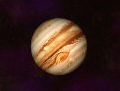
\includegraphics[width=0.8\linewidth]{images/Tc/p1/im1.png}\\
					كوكب المشتري

					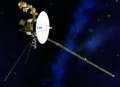
\includegraphics[width=0.8\linewidth]{images/Tc/p1/im2.png}\\
					المسبار 
					Voyager1
					\end{center}
					\end{minipage}
					\end{exercice}%=== source ===%
  %Exercice 17
\begin{exercice}{}/
					يمثل المبيان التالي تغيرات وزن جسم بدلالة كتلته على سطح الأرض (النقط بالأزرق)، وعلى سطح القمر (النقط بالأحمر):
					\begin{center}
					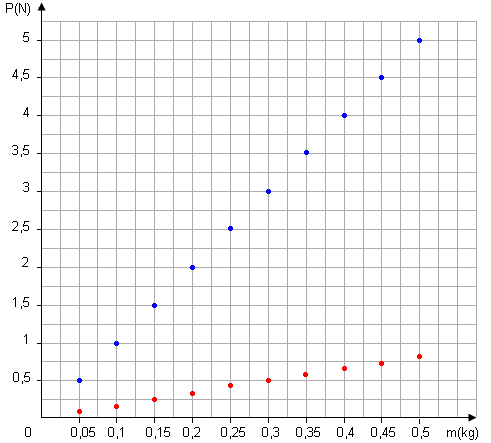
\includegraphics[width=0.6\linewidth]{images/Tc/p1/im3.png}
					\end{center}
					باستغلال المبيان :
					\begin{enumerate}[label=\protect\circled{\color{white}\textbf{\arabic*}}]
					\item بين أن وزن جسم يتناسب اطرادا مع كتلته.
					\item حدد شدة الثقالة على سطح الأرض، وعلى سطح القمر، ثم قارن بينهما.
					\end{enumerate}
					\end{exercice}%=== source ===%  
  %Exercice 18
\begin{exercice}{}/
					بعد مضي قرن على قانون نيوتن للتجاذب الكوني، تمكن العالم كافنديش 
					Cavendish 
					من قياس قيمة ثابتة التجاذب الكوني، حيث وجد 
					{$G=6,754.10^{-11}N.m^2.kg^{-2}$}.
					وبعد ذلك استعمل هذه النتيجة لحساب كتلة الأرض. لنبين كيف فيما  يلي.\\
					يعطي الجدول التالي قيم أوزان أجسام ذات كتل مختلفة على سطح الأرض :
					\begin{center}
					 \begin{tabular}{|c|c|c|c|c|}
					 \hline 
					 2,013 & 1,456 & 0,943 & 0,456 & $m(Kg)$ \\
					 \hline 
					 19,75 & 14,28 & 9,25 & 4,47 & $P(N)$ \\
					 \hline 
					 \end{tabular} 
					 \end{center} 
					 \begin{enumerate}[label=\protect\circled{\color{white}\textbf{\arabic*}}]
					 \item إستنتج من هذه المعطيات قيمة شدة الثقالة 
					 $g$
					 على سطح الأرض.
					 \item عبر بدلالة 
					 $M$
					 كتلة الأرض وشعاعها
					 $R$،
					 عن 
					$F$ 
					 شدة التجاذب المطبقة من طرف الأرض على جسم كتلته 
					 $m$
					 وضع على سطح الأرض.
					\item إستنتج تعبير 
					$g$
					شدة الثقالة على سطح الأرض بدلالة 
					$M$
					و
					$R$.
					ثم تعبير كتلة الأرض بدلالة 
					$g$
					و
					$R$.
					\item علما أن قيمة شعاع الأرض كانت قد حددت من قبل 
					{$R=6,4.10^3Km$}
					وكانت معلومة لدى كافنديش، إستنتج القيمة التي وجدها كافنديش لكتلة الأرض.
					 \end{enumerate}
					\end{exercice}%=== source ===%  
  %Exercice 19
\begin{exercice}{}/
					في مارس من العام 1979 مر المسبار الفضائي 
					voyager1
					بالقرب من كوكب المشتري. يمثل الشكل التالي مسار هذا المسبار.
					\begin{center}
					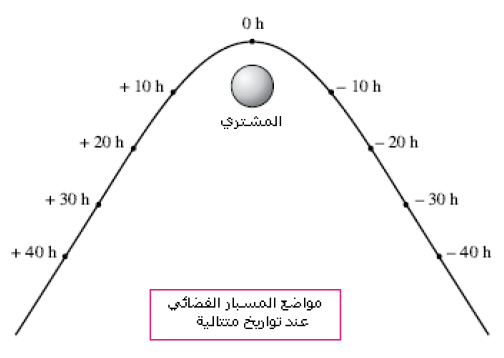
\includegraphics[width=0.5\linewidth]{images/Tc/p1/im4.png}
					\end{center}
					\begin{enumerate}[label=\protect\circled{\color{white}\textbf{\arabic*}}]
					\item ما سبب تغير مسار المسبار الفضائي؟
					\item هل يخضع المسبار لقوة تخاذب أم تنافر؟
					\item هل تتعلق شدة هذه القوة بالمسافة الفاصلة بين المسبار وكوكب المشتري؟
					\item  في أي لحظة تكون شدة هذه القوى قصوى؟
					\item ماذا يحدث للمسبار في حالة مروره بالقرب من المشتري بسرعة ضعيفة؟
					\end{enumerate}
					\end{exercice}%=== source ===%  
  %Exercice 21
\begin{exercice}{}/
					شدة وزن شخص 
					$P_0=700\ N$
					على مستوى سطح البحر، حيث ضدة الثقالة 
					$g_0=9,8N/kg$.
					\begin{enumerate}[label=\protect\circled{\color{white}\textbf{\arabic*}}]
					\item أحسب 
					$m$
					كتلة هذا الشخص.
					\item أحسب شدة وزنه على ارتفاع 
					$h=8882m$.
					\end{enumerate}
					معطيات :
					\begin{itemize}
					\item شعاع الأرض \hrulefill 
					$R_T=6400km$
					\item كتلة الأرض \hrulefill
					$M_T=5,98.10^{24}kg$
					\item ثابتة التجاذب الكوني \hrulefill
					$G=6,67.10^{-11}N.m^2.kg^{-2}$.
					\end{itemize}
					\end{exercice}%=== source ===%
  %Exercice 20
\begin{exercice}{}/
					في مبارة للكرة الحديدية، توقفت الكرة الحديدية على مسافة 
					$20cm$
					من البولينغ (أو الجاك).
					\begin{center}
\begin{adjustbox}{width=0.4\linewidth}
\fbox{
					\psset{xunit=.5pt,yunit=.5pt,runit=.5pt}
\begin{pspicture}(524,344)
{
\newrgbcolor{curcolor}{1 1 1}
\pscustom[linewidth=1,linecolor=curcolor]
{
\newpath
\moveto(1,104)
\lineto(502,104)
\lineto(502,92)
\lineto(1,92)
\closepath
}
}
{
\newrgbcolor{curcolor}{0 0 0}
\pscustom[linewidth=1,linecolor=curcolor]
{
\newpath
\moveto(3.95,104)
\lineto(502.05,104)
}
}
{
\newrgbcolor{curcolor}{0.68627453 0.68627453 0.68627453}
\pscustom[linestyle=none,fillstyle=solid,fillcolor=curcolor]
{
\newpath
\moveto(1,204.95)
\curveto(1,259.85)(45.4,304.25)(100.3,304.25)
\curveto(155.1,304.25)(199.5,259.85)(199.5,204.95)
\curveto(199.5,150.15)(155.1,105.75)(100.3,105.75)
\curveto(45.4,105.75)(1,150.15)(1,204.95)
\closepath
}
}
{
\newrgbcolor{curcolor}{0 0 0}
\pscustom[linewidth=1,linecolor=curcolor]
{
\newpath
\moveto(1,204.95)
\curveto(1,259.85)(45.4,304.25)(100.3,304.25)
\curveto(155.1,304.25)(199.5,259.85)(199.5,204.95)
\curveto(199.5,150.15)(155.1,105.75)(100.3,105.75)
\curveto(45.4,105.75)(1,150.15)(1,204.95)
\closepath
}
}
{
\newrgbcolor{curcolor}{0.93333334 0.48627451 0.19215687}
\pscustom[linestyle=none,fillstyle=solid,fillcolor=curcolor]
{
\newpath
\moveto(425.75,138.9)
\curveto(425.75,157.2)(440.55,172)(458.85,172)
\curveto(477.15,172)(492.05,157.2)(492.05,138.9)
\curveto(492.05,120.6)(477.15,105.7)(458.85,105.7)
\curveto(440.55,105.7)(425.75,120.6)(425.75,138.9)
\closepath
}
}
{
\newrgbcolor{curcolor}{0 0 0}
\pscustom[linewidth=1,linecolor=curcolor]
{
\newpath
\moveto(425.75,138.9)
\curveto(425.75,157.2)(440.55,172)(458.85,172)
\curveto(477.15,172)(492.05,157.2)(492.05,138.9)
\curveto(492.05,120.6)(477.15,105.7)(458.85,105.7)
\curveto(440.55,105.7)(425.75,120.6)(425.75,138.9)
\closepath
}
}
{
\newrgbcolor{curcolor}{0 0 0}
\pscustom[linewidth=3,linecolor=curcolor,linestyle=dashed,dash=6 4]
{
\newpath
\moveto(100,205)
\lineto(100,26)
}
}
{
\newrgbcolor{curcolor}{0 0 0}
\pscustom[linewidth=3,linecolor=curcolor,linestyle=dashed,dash=6 4]
{
\newpath
\moveto(459,139)
\lineto(459,26)
}
}
{
\newrgbcolor{curcolor}{0 0 0}
\pscustom[linewidth=3,linecolor=curcolor]
{
\newpath
\moveto(450,32)
\lineto(109,32)
}
}
{
\newrgbcolor{curcolor}{0 0 0}
\pscustom[linestyle=none,fillstyle=solid,fillcolor=curcolor]
{
\newpath
\moveto(459,32)
\lineto(441,37.2)
\lineto(450,32)
\lineto(441,26.8)
\lineto(459,32)
}
}
{
\newrgbcolor{curcolor}{0 0 0}
\pscustom[linewidth=1,linecolor=curcolor]
{
\newpath
\moveto(459,32)
\lineto(441,37.2)
\lineto(450,32)
\lineto(441,26.8)
\lineto(459,32)
}
}
{
\newrgbcolor{curcolor}{0 0 0}
\pscustom[linestyle=none,fillstyle=solid,fillcolor=curcolor]
{
\newpath
\moveto(100,32)
\lineto(118,26.8)
\lineto(109,32)
\lineto(118,37.2)
\lineto(100,32)
}
}
{
\newrgbcolor{curcolor}{0 0 0}
\pscustom[linewidth=1,linecolor=curcolor]
{
\newpath
\moveto(100,32)
\lineto(118,26.8)
\lineto(109,32)
\lineto(118,37.2)
\lineto(100,32)
}
}
{
\newrgbcolor{curcolor}{0 0 0}
\pscustom[linestyle=none,fillstyle=solid,fillcolor=curcolor]
{
\newpath
\moveto(235.13671875,10)
\lineto(232.078125,10)
\lineto(232.078125,11.828125)
\curveto(231.5703125,11.1171875)(230.96875,10.5859375)(230.2734375,10.234375)
\curveto(229.5859375,9.890625)(228.890625,9.71875)(228.1875,9.71875)
\curveto(226.7578125,9.71875)(225.53125,10.29296875)(224.5078125,11.44140625)
\curveto(223.4921875,12.59765625)(222.984375,14.20703125)(222.984375,16.26953125)
\curveto(222.984375,18.37890625)(223.48046875,19.98046875)(224.47265625,21.07421875)
\curveto(225.46484375,22.17578125)(226.71875,22.7265625)(228.234375,22.7265625)
\curveto(229.625,22.7265625)(230.828125,22.1484375)(231.84375,20.9921875)
\lineto(231.84375,27.1796875)
\lineto(235.13671875,27.1796875)
\closepath
\moveto(226.34765625,16.4921875)
\curveto(226.34765625,15.1640625)(226.53125,14.203125)(226.8984375,13.609375)
\curveto(227.4296875,12.75)(228.171875,12.3203125)(229.125,12.3203125)
\curveto(229.8828125,12.3203125)(230.52734375,12.640625)(231.05859375,13.28125)
\curveto(231.58984375,13.9296875)(231.85546875,14.89453125)(231.85546875,16.17578125)
\curveto(231.85546875,17.60546875)(231.59765625,18.6328125)(231.08203125,19.2578125)
\curveto(230.56640625,19.890625)(229.90625,20.20703125)(229.1015625,20.20703125)
\curveto(228.3203125,20.20703125)(227.6640625,19.89453125)(227.1328125,19.26953125)
\curveto(226.609375,18.65234375)(226.34765625,17.7265625)(226.34765625,16.4921875)
\closepath
}
}
{
\newrgbcolor{curcolor}{0 0 0}
\pscustom[linestyle=none,fillstyle=solid,fillcolor=curcolor]
{
\newpath
\moveto(244.32421875,19.5625)
\lineto(244.32421875,22.5859375)
\lineto(256.3359375,22.5859375)
\lineto(256.3359375,19.5625)
\closepath
\moveto(244.32421875,14.359375)
\lineto(244.32421875,17.39453125)
\lineto(256.3359375,17.39453125)
\lineto(256.3359375,14.359375)
\closepath
}
}
{
\newrgbcolor{curcolor}{0 0 0}
\pscustom[linestyle=none,fillstyle=solid,fillcolor=curcolor]
{
\newpath
\moveto(276.140625,13.05859375)
\lineto(276.140625,10)
\lineto(264.59765625,10)
\curveto(264.72265625,11.15625)(265.09765625,12.25)(265.72265625,13.28125)
\curveto(266.34765625,14.3203125)(267.58203125,15.6953125)(269.42578125,17.40625)
\curveto(270.91015625,18.7890625)(271.8203125,19.7265625)(272.15625,20.21875)
\curveto(272.609375,20.8984375)(272.8359375,21.5703125)(272.8359375,22.234375)
\curveto(272.8359375,22.96875)(272.63671875,23.53125)(272.23828125,23.921875)
\curveto(271.84765625,24.3203125)(271.3046875,24.51953125)(270.609375,24.51953125)
\curveto(269.921875,24.51953125)(269.375,24.3125)(268.96875,23.8984375)
\curveto(268.5625,23.484375)(268.328125,22.796875)(268.265625,21.8359375)
\lineto(264.984375,22.1640625)
\curveto(265.1796875,23.9765625)(265.79296875,25.27734375)(266.82421875,26.06640625)
\curveto(267.85546875,26.85546875)(269.14453125,27.25)(270.69140625,27.25)
\curveto(272.38671875,27.25)(273.71875,26.79296875)(274.6875,25.87890625)
\curveto(275.65625,24.96484375)(276.140625,23.828125)(276.140625,22.46875)
\curveto(276.140625,21.6953125)(276,20.95703125)(275.71875,20.25390625)
\curveto(275.4453125,19.55859375)(275.0078125,18.828125)(274.40625,18.0625)
\curveto(274.0078125,17.5546875)(273.2890625,16.82421875)(272.25,15.87109375)
\curveto(271.2109375,14.91796875)(270.55078125,14.28515625)(270.26953125,13.97265625)
\curveto(269.99609375,13.66015625)(269.7734375,13.35546875)(269.6015625,13.05859375)
\closepath
}
}
{
\newrgbcolor{curcolor}{0 0 0}
\pscustom[linestyle=none,fillstyle=solid,fillcolor=curcolor]
{
\newpath
\moveto(283.9453125,27.25)
\curveto(285.609375,27.25)(286.91015625,26.65625)(287.84765625,25.46875)
\curveto(288.96484375,24.0625)(289.5234375,21.73046875)(289.5234375,18.47265625)
\curveto(289.5234375,15.22265625)(288.9609375,12.88671875)(287.8359375,11.46484375)
\curveto(286.90625,10.29296875)(285.609375,9.70703125)(283.9453125,9.70703125)
\curveto(282.2734375,9.70703125)(280.92578125,10.34765625)(279.90234375,11.62890625)
\curveto(278.87890625,12.91796875)(278.3671875,15.2109375)(278.3671875,18.5078125)
\curveto(278.3671875,21.7421875)(278.9296875,24.0703125)(280.0546875,25.4921875)
\curveto(280.984375,26.6640625)(282.28125,27.25)(283.9453125,27.25)
\closepath
\moveto(283.9453125,24.51953125)
\curveto(283.546875,24.51953125)(283.19140625,24.390625)(282.87890625,24.1328125)
\curveto(282.56640625,23.8828125)(282.32421875,23.4296875)(282.15234375,22.7734375)
\curveto(281.92578125,21.921875)(281.8125,20.48828125)(281.8125,18.47265625)
\curveto(281.8125,16.45703125)(281.9140625,15.0703125)(282.1171875,14.3125)
\curveto(282.3203125,13.5625)(282.57421875,13.0625)(282.87890625,12.8125)
\curveto(283.19140625,12.5625)(283.546875,12.4375)(283.9453125,12.4375)
\curveto(284.34375,12.4375)(284.69921875,12.5625)(285.01171875,12.8125)
\curveto(285.32421875,13.0703125)(285.56640625,13.52734375)(285.73828125,14.18359375)
\curveto(285.96484375,15.02734375)(286.078125,16.45703125)(286.078125,18.47265625)
\curveto(286.078125,20.48828125)(285.9765625,21.87109375)(285.7734375,22.62109375)
\curveto(285.5703125,23.37890625)(285.3125,23.8828125)(285,24.1328125)
\curveto(284.6953125,24.390625)(284.34375,24.51953125)(283.9453125,24.51953125)
\closepath
}
}
{
\newrgbcolor{curcolor}{0 0 0}
\pscustom[linestyle=none,fillstyle=solid,fillcolor=curcolor]
{
\newpath
\moveto(309.94921875,18.765625)
\lineto(306.703125,18.1796875)
\curveto(306.59375,18.828125)(306.34375,19.31640625)(305.953125,19.64453125)
\curveto(305.5703125,19.97265625)(305.0703125,20.13671875)(304.453125,20.13671875)
\curveto(303.6328125,20.13671875)(302.9765625,19.8515625)(302.484375,19.28125)
\curveto(302,18.71875)(301.7578125,17.7734375)(301.7578125,16.4453125)
\curveto(301.7578125,14.96875)(302.00390625,13.92578125)(302.49609375,13.31640625)
\curveto(302.99609375,12.70703125)(303.6640625,12.40234375)(304.5,12.40234375)
\curveto(305.125,12.40234375)(305.63671875,12.578125)(306.03515625,12.9296875)
\curveto(306.43359375,13.2890625)(306.71484375,13.90234375)(306.87890625,14.76953125)
\lineto(310.11328125,14.21875)
\curveto(309.77734375,12.734375)(309.1328125,11.61328125)(308.1796875,10.85546875)
\curveto(307.2265625,10.09765625)(305.94921875,9.71875)(304.34765625,9.71875)
\curveto(302.52734375,9.71875)(301.07421875,10.29296875)(299.98828125,11.44140625)
\curveto(298.91015625,12.58984375)(298.37109375,14.1796875)(298.37109375,16.2109375)
\curveto(298.37109375,18.265625)(298.9140625,19.86328125)(300,21.00390625)
\curveto(301.0859375,22.15234375)(302.5546875,22.7265625)(304.40625,22.7265625)
\curveto(305.921875,22.7265625)(307.125,22.3984375)(308.015625,21.7421875)
\curveto(308.9140625,21.09375)(309.55859375,20.1015625)(309.94921875,18.765625)
\closepath
}
}
{
\newrgbcolor{curcolor}{0 0 0}
\pscustom[linestyle=none,fillstyle=solid,fillcolor=curcolor]
{
\newpath
\moveto(312.2109375,22.4453125)
\lineto(315.24609375,22.4453125)
\lineto(315.24609375,20.74609375)
\curveto(316.33203125,22.06640625)(317.625,22.7265625)(319.125,22.7265625)
\curveto(319.921875,22.7265625)(320.61328125,22.5625)(321.19921875,22.234375)
\curveto(321.78515625,21.90625)(322.265625,21.41015625)(322.640625,20.74609375)
\curveto(323.1875,21.41015625)(323.77734375,21.90625)(324.41015625,22.234375)
\curveto(325.04296875,22.5625)(325.71875,22.7265625)(326.4375,22.7265625)
\curveto(327.3515625,22.7265625)(328.125,22.5390625)(328.7578125,22.1640625)
\curveto(329.390625,21.796875)(329.86328125,21.25390625)(330.17578125,20.53515625)
\curveto(330.40234375,20.00390625)(330.515625,19.14453125)(330.515625,17.95703125)
\lineto(330.515625,10)
\lineto(327.22265625,10)
\lineto(327.22265625,17.11328125)
\curveto(327.22265625,18.34765625)(327.109375,19.14453125)(326.8828125,19.50390625)
\curveto(326.578125,19.97265625)(326.109375,20.20703125)(325.4765625,20.20703125)
\curveto(325.015625,20.20703125)(324.58203125,20.06640625)(324.17578125,19.78515625)
\curveto(323.76953125,19.50390625)(323.4765625,19.08984375)(323.296875,18.54296875)
\curveto(323.1171875,18.00390625)(323.02734375,17.1484375)(323.02734375,15.9765625)
\lineto(323.02734375,10)
\lineto(319.734375,10)
\lineto(319.734375,16.8203125)
\curveto(319.734375,18.03125)(319.67578125,18.8125)(319.55859375,19.1640625)
\curveto(319.44140625,19.515625)(319.2578125,19.77734375)(319.0078125,19.94921875)
\curveto(318.765625,20.12109375)(318.43359375,20.20703125)(318.01171875,20.20703125)
\curveto(317.50390625,20.20703125)(317.046875,20.0703125)(316.640625,19.796875)
\curveto(316.234375,19.5234375)(315.94140625,19.12890625)(315.76171875,18.61328125)
\curveto(315.58984375,18.09765625)(315.50390625,17.2421875)(315.50390625,16.046875)
\lineto(315.50390625,10)
\lineto(312.2109375,10)
\closepath
}
}
{
\newrgbcolor{curcolor}{0 0 0}
\pscustom[linewidth=2.98918049,linecolor=curcolor,linestyle=dashed,dash=6 4]
{
\newpath
\moveto(100,205)
\lineto(457.7,139.3)
}
}
{
\newrgbcolor{curcolor}{0 0 0}
\pscustom[linestyle=none,fillstyle=solid,fillcolor=curcolor]
{
\newpath
\moveto(153.44264678,323.16760351)
\curveto(153.44264678,322.54954794)(153.36973011,321.9835757)(153.22389678,321.4696868)
\curveto(153.07806344,320.96274234)(152.79681343,320.27871454)(152.38014675,319.4176034)
\lineto(151.75514673,319.66760341)
\curveto(151.9218134,320.55649233)(152.00514674,321.27871457)(152.00514674,321.83427014)
\curveto(152.00514674,322.25788127)(151.97042452,322.87940906)(151.90098007,323.69885353)
\curveto(151.83153562,324.518298)(151.74473006,325.3273258)(151.64056339,326.12593694)
\curveto(151.53639672,326.93149252)(151.36625783,327.88982588)(151.13014671,329.00093702)
\curveto(151.04681338,329.38982592)(151.00514671,329.65718704)(151.00514671,329.80302038)
\curveto(151.00514671,330.01829816)(151.1127856,330.38288151)(151.32806339,330.89677041)
\curveto(151.54334117,331.41760376)(151.84542451,332.046076)(152.23431341,332.78218713)
\lineto(152.85931343,329.09468702)
\curveto(153.0884801,327.69190921)(153.24820233,326.47663139)(153.33848011,325.44885358)
\curveto(153.40792456,324.65718689)(153.44264678,323.8967702)(153.44264678,323.16760351)
\closepath
}
}
{
\newrgbcolor{curcolor}{0 0 0}
\pscustom[linestyle=none,fillstyle=solid,fillcolor=curcolor]
{
\newpath
\moveto(149.58848015,320.13635342)
\lineto(143.85931331,320.13635342)
\lineto(143.85931331,322.96968684)
\lineto(148.33848011,322.96968684)
\lineto(147.07806341,330.04260372)
\lineto(146.41139672,330.48010373)
\curveto(146.41139672,330.88982597)(146.47389672,331.30302042)(146.59889673,331.7196871)
\curveto(146.75861895,332.2474649)(147.02945229,332.87593714)(147.41139675,333.60510383)
\lineto(147.89056343,333.35510382)
\curveto(147.89056343,333.31343715)(147.87667454,333.20232604)(147.84889676,333.02177047)
\curveto(147.84889676,332.7926038)(147.9947301,332.57038157)(148.28639678,332.35510379)
\curveto(148.54334123,332.16065934)(148.95306346,331.94538155)(149.51556348,331.70927044)
\curveto(149.45306348,331.26482598)(149.35931348,330.83079819)(149.23431347,330.40718706)
\curveto(149.11625791,329.98357594)(148.98084124,329.60510371)(148.82806346,329.27177036)
\lineto(148.45306345,329.4176037)
\lineto(149.58848015,322.96968684)
\closepath
}
}
{
\newrgbcolor{curcolor}{0 0 0}
\pscustom[linestyle=none,fillstyle=solid,fillcolor=curcolor]
{
\newpath
\moveto(144.56764435,320.13635342)
\lineto(136.15097744,320.13635342)
\lineto(136.15097744,322.96968684)
\lineto(142.9113943,322.96968684)
\curveto(142.64056096,323.29607574)(142.37667207,323.58079797)(142.11972761,323.82385353)
\curveto(141.91139427,324.01829798)(141.63014427,324.2544091)(141.27597759,324.53218689)
\curveto(140.88014424,324.83774245)(140.48778312,325.14329802)(140.09889422,325.44885358)
\lineto(139.76556088,325.07385357)
\curveto(139.1475053,325.6849647)(138.77944974,326.05649249)(138.66139418,326.18843694)
\curveto(138.31417194,326.58427028)(138.14056083,327.03913141)(138.14056083,327.55302031)
\curveto(138.14056083,328.25440922)(138.18917194,328.74746479)(138.28639417,329.03218702)
\curveto(138.42528306,329.43496481)(138.72042196,329.79260371)(139.17181086,330.10510372)
\curveto(139.57458865,330.38288151)(140.00514422,330.63635374)(140.46347756,330.86552041)
\curveto(140.82458869,331.04607597)(141.30375537,331.25788153)(141.90097761,331.5009371)
\curveto(142.17875539,331.61204821)(142.76556097,331.84121488)(143.66139433,332.18843712)
\lineto(143.66139433,329.70927038)
\curveto(143.6266721,329.70927038)(143.33500543,329.6189926)(142.7863943,329.43843703)
\curveto(142.10583872,329.21621481)(141.56417204,329.02177036)(141.16139425,328.85510368)
\curveto(140.5780609,328.61899257)(140.28639423,328.44190923)(140.28639423,328.32385367)
\curveto(140.28639423,328.26135367)(140.53292201,327.99052033)(141.02597758,327.51135364)
\curveto(141.69958871,326.85857585)(142.26556095,326.26135361)(142.7238943,325.71968692)
\curveto(143.48083876,324.82385356)(144.09542212,323.93149243)(144.56764435,323.04260351)
\closepath
}
}
{
\newrgbcolor{curcolor}{0 0 0}
\pscustom[linestyle=none,fillstyle=solid,fillcolor=curcolor]
{
\newpath
\moveto(136.85931869,319.89677008)
\curveto(136.85931869,319.47315896)(136.61626313,318.91065894)(136.13015201,318.20927003)
\curveto(135.64404088,317.51482557)(135.07459642,316.91065888)(134.42181862,316.39676998)
\curveto(133.69959638,315.82732552)(133.0815408,315.54260329)(132.5676519,315.54260329)
\curveto(131.95654077,315.54260329)(131.30029075,315.7162144)(130.59890184,316.06343664)
\curveto(129.98779071,316.36204776)(129.03292957,316.95927)(127.73431842,317.85510336)
\lineto(128.17181844,318.50093671)
\curveto(128.79681845,318.08427003)(129.30029069,317.80302002)(129.68223515,317.65718668)
\curveto(130.0641796,317.51135335)(130.47737406,317.43843668)(130.92181852,317.43843668)
\curveto(131.4009852,317.43843668)(131.88015188,317.57385335)(132.35931856,317.84468669)
\curveto(132.83848524,318.11552003)(133.49126304,318.61899227)(134.31765195,319.3551034)
\curveto(135.47042976,320.38288121)(136.04681867,321.1745479)(136.04681867,321.73010347)
\curveto(136.04681867,322.00788126)(135.93570756,322.3724646)(135.71348533,322.8238535)
\curveto(135.46348532,323.33774241)(135.15792976,323.76482575)(134.79681863,324.10510354)
\lineto(135.38015198,326.91760363)
\curveto(135.85237422,326.4314925)(136.21695756,325.87246471)(136.47390202,325.24052024)
\curveto(136.73084647,324.60857578)(136.85931869,323.88982576)(136.85931869,323.08427018)
\closepath
}
}
{
\newrgbcolor{curcolor}{0 0 0}
\pscustom[linestyle=none,fillstyle=solid,fillcolor=curcolor]
{
\newpath
\moveto(126.2551532,332.30302045)
\lineto(125.10931983,330.17802039)
\lineto(123.63015312,331.01135375)
\lineto(122.79681977,329.36552037)
\lineto(120.85931971,330.4280204)
\lineto(121.94265307,332.44885379)
\lineto(123.48431979,331.67802043)
\lineto(124.35931981,333.36552049)
\closepath
\moveto(126.77598655,324.04260354)
\curveto(126.77598655,323.62593686)(126.74126433,323.20232574)(126.67181988,322.77177017)
\curveto(126.60931988,322.34815905)(126.52598654,322.00093681)(126.42181987,321.73010347)
\curveto(126.22737542,321.20232568)(125.74820874,320.73704789)(124.98431983,320.3342701)
\curveto(124.27598648,319.95927009)(123.60931979,319.77177008)(122.98431977,319.77177008)
\curveto(122.44265309,319.77177008)(122.01209752,319.95927009)(121.69265307,320.3342701)
\curveto(121.37320861,320.70927011)(121.21348639,321.20927012)(121.21348639,321.83427014)
\curveto(121.21348639,322.4037146)(121.2933475,322.9627424)(121.45306973,323.51135352)
\curveto(121.6197364,324.05996465)(121.91487529,324.7509369)(122.33848642,325.58427025)
\lineto(121.96348641,325.83427026)
\curveto(122.08154197,326.15371471)(122.24126419,326.53913139)(122.44265309,326.9905203)
\curveto(122.64404198,327.44885364)(122.82459754,327.83427032)(122.98431977,328.14677033)
\lineto(124.00515314,327.54260365)
\curveto(124.44959759,327.2717703)(124.87320872,326.98010363)(125.27598651,326.66760362)
\curveto(125.84543097,326.23704805)(126.23779209,325.83079804)(126.45306987,325.44885358)
\curveto(126.66834766,325.07385357)(126.77598655,324.60510356)(126.77598655,324.04260354)
\closepath
\moveto(125.23431984,323.20927018)
\curveto(125.23431984,323.34121463)(124.99126428,323.61552019)(124.50515315,324.03218687)
\curveto(124.02598647,324.44885355)(123.55376423,324.80649245)(123.08848644,325.10510357)
\curveto(122.64404198,324.40371466)(122.42181975,323.82038131)(122.42181975,323.35510352)
\curveto(122.42181975,323.13288129)(122.51209753,322.94190906)(122.6926531,322.78218684)
\curveto(122.8801531,322.62246461)(123.10237533,322.5426035)(123.35931978,322.5426035)
\curveto(123.70654202,322.5426035)(124.10584758,322.62246461)(124.55723648,322.78218684)
\curveto(125.00862539,322.94885351)(125.23431984,323.09121462)(125.23431984,323.20927018)
\closepath
}
}
{
\newrgbcolor{curcolor}{0 0 0}
\pscustom[linestyle=none,fillstyle=solid,fillcolor=curcolor]
{
\newpath
\moveto(113.60931472,323.16760351)
\curveto(113.60931472,322.54954794)(113.53639805,321.9835757)(113.39056471,321.4696868)
\curveto(113.24473138,320.96274234)(112.96348137,320.27871454)(112.54681469,319.4176034)
\lineto(111.92181467,319.66760341)
\curveto(112.08848134,320.55649233)(112.17181468,321.27871457)(112.17181468,321.83427014)
\curveto(112.17181468,322.25788127)(112.13709245,322.87940906)(112.06764801,323.69885353)
\curveto(111.99820356,324.518298)(111.911398,325.3273258)(111.80723133,326.12593694)
\curveto(111.70306466,326.93149252)(111.53292577,327.88982588)(111.29681465,329.00093702)
\curveto(111.21348132,329.38982592)(111.17181465,329.65718704)(111.17181465,329.80302038)
\curveto(111.17181465,330.01829816)(111.27945354,330.38288151)(111.49473132,330.89677041)
\curveto(111.71000911,331.41760376)(112.01209245,332.046076)(112.40098135,332.78218713)
\lineto(113.02598137,329.09468702)
\curveto(113.25514804,327.69190921)(113.41487027,326.47663139)(113.50514805,325.44885358)
\curveto(113.5745925,324.65718689)(113.60931472,323.8967702)(113.60931472,323.16760351)
\closepath
}
}
{
\newrgbcolor{curcolor}{0 0 0}
\pscustom[linestyle=none,fillstyle=solid,fillcolor=curcolor]
{
\newpath
\moveto(109.75514809,320.13635342)
\lineto(104.02598125,320.13635342)
\lineto(104.02598125,322.96968684)
\lineto(108.50514805,322.96968684)
\lineto(107.24473135,330.04260372)
\lineto(106.57806466,330.48010373)
\curveto(106.57806466,330.88982597)(106.64056466,331.30302042)(106.76556466,331.7196871)
\curveto(106.92528689,332.2474649)(107.19612023,332.87593714)(107.57806469,333.60510383)
\lineto(108.05723137,333.35510382)
\curveto(108.05723137,333.31343715)(108.04334248,333.20232604)(108.0155647,333.02177047)
\curveto(108.0155647,332.7926038)(108.16139804,332.57038157)(108.45306472,332.35510379)
\curveto(108.71000917,332.16065934)(109.1197314,331.94538155)(109.68223142,331.70927044)
\curveto(109.61973142,331.26482598)(109.52598141,330.83079819)(109.40098141,330.40718706)
\curveto(109.28292585,329.98357594)(109.14750918,329.60510371)(108.9947314,329.27177036)
\lineto(108.61973139,329.4176037)
\lineto(109.75514809,322.96968684)
\closepath
}
}
{
\newrgbcolor{curcolor}{0 0 0}
\pscustom[linestyle=none,fillstyle=solid,fillcolor=curcolor]
{
\newpath
\moveto(104.755147,320.13635342)
\lineto(92.85931331,320.13635342)
\lineto(92.85931331,322.96968684)
\lineto(100.26556353,322.96968684)
\curveto(99.42528573,323.83774242)(98.64750793,324.46274244)(97.93223013,324.8446869)
\curveto(97.30028567,325.18496469)(96.68223009,325.35510358)(96.07806341,325.35510358)
\curveto(95.89750785,325.35510358)(95.73084117,325.34468691)(95.57806339,325.32385358)
\curveto(95.43223005,325.30996469)(95.21695227,325.27177024)(94.93223004,325.20927024)
\curveto(95.3141745,326.08427027)(95.73778562,326.73010362)(96.20306341,327.1467703)
\curveto(96.67528565,327.56343698)(97.21000789,327.77177032)(97.80723013,327.77177032)
\curveto(98.26556347,327.77177032)(98.70653571,327.6606592)(99.13014683,327.43843698)
\curveto(99.55375796,327.21621475)(100.02945241,326.85857585)(100.55723021,326.36552028)
\curveto(100.97389689,325.97663138)(101.56417468,325.36899247)(102.32806359,324.54260356)
\curveto(102.84889694,323.9592702)(103.24473029,323.58079797)(103.51556363,323.40718686)
\curveto(103.79334142,323.23357574)(104.20653587,323.0877424)(104.755147,322.96968684)
\closepath
}
}
{
\newrgbcolor{curcolor}{0 0 0}
\pscustom[linestyle=none,fillstyle=solid,fillcolor=curcolor]
{
\newpath
\moveto(93.56764625,320.13635342)
\lineto(88.84889611,320.13635342)
\curveto(88.39056276,320.13635342)(88.03986831,320.23357565)(87.79681274,320.4280201)
\curveto(87.49820162,320.66413122)(87.34889606,321.0495479)(87.34889606,321.58427013)
\curveto(87.34889606,321.8898257)(87.36278495,322.21968682)(87.39056273,322.5738535)
\curveto(87.42528495,322.92802017)(87.47389607,323.28565907)(87.53639607,323.6467702)
\lineto(87.93222941,323.66760353)
\curveto(87.98778497,323.42454797)(88.10931275,323.24746463)(88.29681276,323.13635351)
\curveto(88.49125721,323.0252424)(88.7238961,322.96968684)(88.99472945,322.96968684)
\lineto(92.57806289,322.96968684)
\curveto(92.41834066,323.99052021)(92.14056287,324.80649245)(91.74472953,325.41760358)
\curveto(91.41834063,325.92454804)(90.9634795,326.36204805)(90.38014615,326.73010362)
\lineto(91.13014618,329.98010372)
\curveto(92.03292398,329.30649259)(92.67181289,328.43843701)(93.0468129,327.37593697)
\curveto(93.39403513,326.39677028)(93.56764625,325.09815913)(93.56764625,323.48010352)
\closepath
}
}
{
\newrgbcolor{curcolor}{0 0 0}
\pscustom[linestyle=none,fillstyle=solid,fillcolor=curcolor]
{
\newpath
\moveto(86.25514875,320.13635342)
\lineto(79.73431522,320.13635342)
\lineto(79.73431522,322.96968684)
\lineto(85.21348205,322.96968684)
\curveto(85.13709316,323.44190908)(84.99820426,323.84121465)(84.79681537,324.16760354)
\curveto(84.6926487,324.34815911)(84.44959314,324.66065911)(84.06764868,325.10510357)
\lineto(84.90098204,327.58427031)
\curveto(85.42181539,326.99399252)(85.77598207,326.37593694)(85.96348207,325.73010359)
\curveto(86.15792652,325.08427024)(86.25514875,324.12593688)(86.25514875,322.85510351)
\closepath
\moveto(86.08848207,318.30302004)
\lineto(84.94264871,316.17801997)
\lineto(83.463482,317.01135333)
\lineto(82.63014864,315.36551995)
\lineto(80.69264858,316.42801998)
\lineto(81.77598195,318.44885337)
\lineto(83.31764866,317.67802002)
\lineto(84.19264869,319.36552007)
\closepath
}
}
{
\newrgbcolor{curcolor}{0 0 0}
\pscustom[linestyle=none,fillstyle=solid,fillcolor=curcolor]
{
\newpath
\moveto(80.44264816,320.13635342)
\lineto(75.72389802,320.13635342)
\curveto(75.26556467,320.13635342)(74.91487021,320.23357565)(74.67181465,320.4280201)
\curveto(74.37320353,320.66413122)(74.22389797,321.0495479)(74.22389797,321.58427013)
\curveto(74.22389797,321.8898257)(74.23778686,322.21968682)(74.26556464,322.5738535)
\curveto(74.30028686,322.92802017)(74.34889797,323.28565907)(74.41139798,323.6467702)
\lineto(74.80723132,323.66760353)
\curveto(74.86278688,323.42454797)(74.98431466,323.24746463)(75.17181467,323.13635351)
\curveto(75.36625912,323.0252424)(75.59889801,322.96968684)(75.86973135,322.96968684)
\lineto(79.45306479,322.96968684)
\curveto(79.29334257,323.99052021)(79.01556478,324.80649245)(78.61973144,325.41760358)
\curveto(78.29334254,325.92454804)(77.83848141,326.36204805)(77.25514806,326.73010362)
\lineto(78.00514808,329.98010372)
\curveto(78.90792589,329.30649259)(79.5468148,328.43843701)(79.92181481,327.37593697)
\curveto(80.26903704,326.39677028)(80.44264816,325.09815913)(80.44264816,323.48010352)
\closepath
}
}
{
\newrgbcolor{curcolor}{0 0 0}
\pscustom[linestyle=none,fillstyle=solid,fillcolor=curcolor]
{
\newpath
\moveto(73.13014779,320.13635342)
\lineto(66.60931427,320.13635342)
\lineto(66.60931427,322.96968684)
\lineto(72.0884811,322.96968684)
\curveto(72.0120922,323.44190908)(71.87320331,323.84121465)(71.67181442,324.16760354)
\curveto(71.56764775,324.34815911)(71.32459218,324.66065911)(70.94264773,325.10510357)
\lineto(71.77598109,327.58427031)
\curveto(72.29681443,326.99399252)(72.65098111,326.37593694)(72.83848112,325.73010359)
\curveto(73.03292557,325.08427024)(73.13014779,324.12593688)(73.13014779,322.85510351)
\closepath
\moveto(72.96348112,318.30302004)
\lineto(71.81764775,316.17801997)
\lineto(70.33848104,317.01135333)
\lineto(69.50514768,315.36551995)
\lineto(67.56764763,316.42801998)
\lineto(68.65098099,318.44885337)
\lineto(70.19264771,317.67802002)
\lineto(71.06764773,319.36552007)
\closepath
}
}
{
\newrgbcolor{curcolor}{0 0 0}
\pscustom[linestyle=none,fillstyle=solid,fillcolor=curcolor]
{
\newpath
\moveto(64.91139755,334.74052053)
\lineto(63.76556418,332.80302047)
\lineto(62.28639747,333.63635383)
\lineto(61.45306411,331.99052044)
\lineto(59.51556405,333.05302048)
\lineto(60.59889742,334.88635386)
\lineto(62.14056413,334.11552051)
\lineto(63.04681416,335.70927056)
\closepath
\moveto(67.31764762,320.13635342)
\lineto(65.95306425,320.13635342)
\curveto(65.70306424,320.13635342)(65.47389756,320.18843676)(65.26556423,320.29260343)
\curveto(64.86278644,320.49399232)(64.52250865,320.86204789)(64.24473086,321.39677013)
\curveto(63.86973085,322.13288126)(63.62667529,323.13982574)(63.51556417,324.41760355)
\curveto(63.04334194,323.8342702)(62.67528637,323.42107574)(62.41139747,323.17802018)
\curveto(62.02945302,322.8238535)(61.71000856,322.64677017)(61.45306411,322.64677017)
\curveto(61.32111966,322.64677017)(61.15445299,322.6676035)(60.9530641,322.70927017)
\lineto(59.68223073,322.95927018)
\curveto(59.14056404,323.07038129)(58.8072307,323.1502424)(58.6822307,323.19885352)
\curveto(58.55723069,323.24746463)(58.49473069,323.33427019)(58.49473069,323.45927019)
\curveto(58.49473069,323.6467702)(58.73431403,324.23704799)(59.21348071,325.23010358)
\curveto(59.69959184,326.23010361)(60.05028629,326.84815918)(60.26556408,327.0842703)
\curveto(60.43917519,327.2717703)(60.74820298,327.51482587)(61.19264744,327.81343699)
\curveto(61.45653633,327.99399255)(61.83153635,328.22663144)(62.31764747,328.51135367)
\lineto(62.86973082,328.83427035)
\curveto(62.84889749,328.93149258)(62.83153637,329.0287148)(62.81764749,329.12593703)
\curveto(62.81070304,329.2301037)(62.80723082,329.32732592)(62.80723082,329.4176037)
\curveto(62.80723082,329.6814926)(62.8662586,330.01135372)(62.98431416,330.40718706)
\curveto(63.10931416,330.80996485)(63.32806417,331.30649265)(63.64056418,331.89677044)
\lineto(64.64056421,325.39677025)
\curveto(64.80028643,324.37593688)(65.00861977,323.68496464)(65.26556423,323.32385352)
\curveto(65.4322309,323.0877424)(65.66139757,322.96968684)(65.95306425,322.96968684)
\lineto(67.31764762,322.96968684)
\closepath
\moveto(63.26556417,326.02177027)
\lineto(63.05723083,327.2717703)
\curveto(62.8350086,327.16760363)(62.66139748,327.0842703)(62.53639748,327.0217703)
\curveto(62.15445302,326.8203814)(61.84889746,326.6328814)(61.61973078,326.45927028)
\curveto(61.45306411,326.32038139)(61.31417522,326.19190916)(61.2030641,326.0738536)
\curveto(61.06417521,325.92107582)(60.99473076,325.80649248)(60.99473076,325.73010359)
\curveto(60.99473076,325.63288137)(61.11625855,325.55649247)(61.35931411,325.50093692)
\curveto(61.60236967,325.44538136)(61.84195301,325.41760358)(62.07806413,325.41760358)
\curveto(62.23084191,325.41760358)(62.39056414,325.45927025)(62.55723081,325.54260359)
\curveto(62.72389748,325.63288137)(62.9600086,325.79260359)(63.26556417,326.02177027)
\closepath
}
}
{
\newrgbcolor{curcolor}{0 0 0}
\pscustom[linestyle=none,fillstyle=solid,fillcolor=curcolor]
{
\newpath
\moveto(499.26553023,189.77680342)
\lineto(490.84886331,189.77680342)
\lineto(490.84886331,192.61013684)
\lineto(497.60928018,192.61013684)
\curveto(497.33844684,192.93652574)(497.07455794,193.22124797)(496.81761349,193.46430353)
\curveto(496.60928015,193.65874798)(496.32803014,193.8948591)(495.97386346,194.17263689)
\curveto(495.57803012,194.47819245)(495.185669,194.78374802)(494.7967801,195.08930358)
\lineto(494.46344675,194.71430357)
\curveto(493.84539118,195.3254147)(493.47733561,195.69694249)(493.35928005,195.82888694)
\curveto(493.01205782,196.22472028)(492.8384467,196.67958141)(492.8384467,197.19347031)
\curveto(492.8384467,197.89485922)(492.88705782,198.38791479)(492.98428004,198.67263702)
\curveto(493.12316893,199.07541481)(493.41830783,199.43305371)(493.86969673,199.74555372)
\curveto(494.27247452,200.02333151)(494.70303009,200.27680374)(495.16136344,200.50597041)
\curveto(495.52247456,200.68652597)(496.00164124,200.89833153)(496.59886348,201.1413871)
\curveto(496.87664127,201.25249821)(497.46344684,201.48166488)(498.3592802,201.82888712)
\lineto(498.3592802,199.34972038)
\curveto(498.32455798,199.34972038)(498.0328913,199.2594426)(497.48428018,199.07888703)
\curveto(496.8037246,198.85666481)(496.26205792,198.66222036)(495.85928013,198.49555368)
\curveto(495.27594678,198.25944257)(494.9842801,198.08235923)(494.9842801,197.96430367)
\curveto(494.9842801,197.90180367)(495.23080789,197.63097033)(495.72386346,197.15180364)
\curveto(496.39747459,196.49902585)(496.96344683,195.90180361)(497.42178017,195.36013692)
\curveto(498.17872464,194.46430356)(498.79330799,193.57194243)(499.26553023,192.68305351)
\closepath
}
}
{
\newrgbcolor{curcolor}{0 0 0}
\pscustom[linestyle=none,fillstyle=solid,fillcolor=curcolor]
{
\newpath
\moveto(491.55719694,189.53722008)
\curveto(491.55719694,189.11360896)(491.31414138,188.55110894)(490.82803025,187.84972003)
\curveto(490.34191913,187.15527557)(489.77247467,186.55110888)(489.11969687,186.03721998)
\curveto(488.39747463,185.46777552)(487.77941905,185.18305329)(487.26553015,185.18305329)
\curveto(486.65441902,185.18305329)(485.998169,185.3566644)(485.29678009,185.70388664)
\curveto(484.68566896,186.00249776)(483.73080782,186.59972)(482.43219667,187.49555336)
\lineto(482.86969668,188.14138671)
\curveto(483.4946967,187.72472003)(483.99816894,187.44347002)(484.38011339,187.29763668)
\curveto(484.76205785,187.15180335)(485.17525231,187.07888668)(485.61969676,187.07888668)
\curveto(486.09886345,187.07888668)(486.57803013,187.21430335)(487.05719681,187.48513669)
\curveto(487.53636349,187.75597003)(488.18914129,188.25944227)(489.0155302,188.9955534)
\curveto(490.16830801,190.02333121)(490.74469692,190.8149979)(490.74469692,191.37055347)
\curveto(490.74469692,191.64833126)(490.6335858,192.0129146)(490.41136357,192.4643035)
\curveto(490.16136357,192.97819241)(489.855808,193.40527575)(489.49469688,193.74555354)
\lineto(490.07803023,196.55805363)
\curveto(490.55025247,196.0719425)(490.91483581,195.51291471)(491.17178026,194.88097024)
\curveto(491.42872472,194.24902578)(491.55719694,193.53027576)(491.55719694,192.72472018)
\closepath
}
}
{
\newrgbcolor{curcolor}{0 0 0}
\pscustom[linestyle=none,fillstyle=solid,fillcolor=curcolor]
{
\newpath
\moveto(480.95303145,201.94347045)
\lineto(479.80719808,199.81847039)
\lineto(478.32803137,200.65180375)
\lineto(477.49469801,199.00597037)
\lineto(475.55719795,200.0684704)
\lineto(476.64053132,202.08930379)
\lineto(478.18219803,201.31847043)
\lineto(479.05719806,203.00597049)
\closepath
\moveto(481.4738648,193.68305354)
\curveto(481.4738648,193.26638686)(481.43914257,192.84277574)(481.36969813,192.41222017)
\curveto(481.30719813,191.98860905)(481.22386479,191.64138681)(481.11969812,191.37055347)
\curveto(480.92525367,190.84277568)(480.44608699,190.37749789)(479.68219808,189.9747201)
\curveto(478.97386472,189.59972009)(478.30719804,189.41222008)(477.68219802,189.41222008)
\curveto(477.14053134,189.41222008)(476.70997577,189.59972009)(476.39053131,189.9747201)
\curveto(476.07108686,190.34972011)(475.91136463,190.84972012)(475.91136463,191.47472014)
\curveto(475.91136463,192.0441646)(475.99122575,192.6031924)(476.15094797,193.15180352)
\curveto(476.31761464,193.70041465)(476.61275354,194.3913869)(477.03636467,195.22472025)
\lineto(476.66136465,195.47472026)
\curveto(476.77942021,195.79416471)(476.93914244,196.17958139)(477.14053134,196.6309703)
\curveto(477.34192023,197.08930364)(477.52247579,197.47472032)(477.68219802,197.78722033)
\lineto(478.70303138,197.18305365)
\curveto(479.14747584,196.9122203)(479.57108696,196.62055363)(479.97386475,196.30805362)
\curveto(480.54330921,195.87749805)(480.93567034,195.47124804)(481.15094812,195.08930358)
\curveto(481.36622591,194.71430357)(481.4738648,194.24555356)(481.4738648,193.68305354)
\closepath
\moveto(479.93219809,192.84972018)
\curveto(479.93219809,192.98166463)(479.68914252,193.25597019)(479.2030314,193.67263687)
\curveto(478.72386472,194.08930355)(478.25164248,194.44694245)(477.78636469,194.74555357)
\curveto(477.34192023,194.04416466)(477.119698,193.46083131)(477.119698,192.99555352)
\curveto(477.119698,192.77333129)(477.20997578,192.58235906)(477.39053134,192.42263684)
\curveto(477.57803135,192.26291461)(477.80025358,192.1830535)(478.05719803,192.1830535)
\curveto(478.40442026,192.1830535)(478.80372583,192.26291461)(479.25511473,192.42263684)
\curveto(479.70650363,192.58930351)(479.93219809,192.73166462)(479.93219809,192.84972018)
\closepath
}
}
{
\newrgbcolor{curcolor}{0 0 0}
\pscustom[linestyle=none,fillstyle=solid,fillcolor=curcolor]
{
\newpath
\moveto(468.30719678,192.80805351)
\curveto(468.30719678,192.18999794)(468.23428011,191.6240257)(468.08844678,191.1101368)
\curveto(467.94261344,190.60319234)(467.66136343,189.91916454)(467.24469675,189.0580534)
\lineto(466.61969673,189.30805341)
\curveto(466.7863634,190.19694233)(466.86969674,190.91916457)(466.86969674,191.47472014)
\curveto(466.86969674,191.89833127)(466.83497452,192.51985906)(466.76553007,193.33930353)
\curveto(466.69608562,194.158748)(466.60928006,194.9677758)(466.50511339,195.76638694)
\curveto(466.40094672,196.57194252)(466.23080783,197.53027588)(465.99469671,198.64138702)
\curveto(465.91136338,199.03027592)(465.86969671,199.29763704)(465.86969671,199.44347038)
\curveto(465.86969671,199.65874816)(465.9773356,200.02333151)(466.19261339,200.53722041)
\curveto(466.40789117,201.05805376)(466.70997451,201.686526)(467.09886341,202.42263713)
\lineto(467.72386343,198.73513702)
\curveto(467.9530301,197.33235921)(468.11275233,196.11708139)(468.20303011,195.08930358)
\curveto(468.27247456,194.29763689)(468.30719678,193.5372202)(468.30719678,192.80805351)
\closepath
}
}
{
\newrgbcolor{curcolor}{0 0 0}
\pscustom[linestyle=none,fillstyle=solid,fillcolor=curcolor]
{
\newpath
\moveto(464.45303015,189.77680342)
\lineto(458.72386331,189.77680342)
\lineto(458.72386331,192.61013684)
\lineto(463.20303011,192.61013684)
\lineto(461.94261341,199.68305372)
\lineto(461.27594672,200.12055373)
\curveto(461.27594672,200.53027597)(461.33844672,200.94347042)(461.46344673,201.3601371)
\curveto(461.62316895,201.8879149)(461.89400229,202.51638714)(462.27594675,203.24555383)
\lineto(462.75511343,202.99555382)
\curveto(462.75511343,202.95388715)(462.74122454,202.84277604)(462.71344676,202.66222047)
\curveto(462.71344676,202.4330538)(462.8592801,202.21083157)(463.15094678,201.99555379)
\curveto(463.40789123,201.80110934)(463.81761346,201.58583155)(464.38011348,201.34972044)
\curveto(464.31761348,200.90527598)(464.22386348,200.47124819)(464.09886347,200.04763706)
\curveto(463.98080791,199.62402594)(463.84539124,199.24555371)(463.69261346,198.91222036)
\lineto(463.31761345,199.0580537)
\lineto(464.45303015,192.61013684)
\closepath
}
}
{
\newrgbcolor{curcolor}{0 0 0}
\pscustom[linestyle=none,fillstyle=solid,fillcolor=curcolor]
{
\newpath
\moveto(459.4530289,189.77680342)
\lineto(452.93219537,189.77680342)
\lineto(452.93219537,192.61013684)
\lineto(458.4113622,192.61013684)
\curveto(458.33497331,193.08235908)(458.19608442,193.48166465)(457.99469552,193.80805354)
\curveto(457.89052885,193.98860911)(457.64747329,194.30110911)(457.26552884,194.74555357)
\lineto(458.09886219,197.22472031)
\curveto(458.61969554,196.63444252)(458.97386222,196.01638694)(459.16136223,195.37055359)
\curveto(459.35580668,194.72472024)(459.4530289,193.76638688)(459.4530289,192.49555351)
\closepath
\moveto(458.39052887,187.57888669)
\lineto(457.14052883,185.24555329)
\lineto(454.72386209,186.55805333)
\lineto(455.97386213,188.9330534)
\closepath
}
}
{
\newrgbcolor{curcolor}{0 0 0}
\pscustom[linestyle=none,fillstyle=solid,fillcolor=curcolor]
{
\newpath
\moveto(453.66136616,190.49555345)
\curveto(453.66136616,189.30110897)(453.1544217,188.12055337)(452.14053278,186.95388667)
\curveto(451.12664387,185.78721997)(450.12664384,185.20388662)(449.1405327,185.20388662)
\curveto(448.56414379,185.20388662)(447.93219933,185.3879144)(447.24469931,185.75596997)
\curveto(446.56414373,186.12402554)(445.51553259,186.84972)(444.09886588,187.93305337)
\lineto(444.53636589,188.53722005)
\curveto(445.28636591,188.03722004)(445.90094927,187.7038867)(446.38011595,187.53722002)
\curveto(446.77594929,187.39833113)(447.22386597,187.32888668)(447.72386599,187.32888668)
\curveto(448.39747712,187.32888668)(449.0641438,187.51638669)(449.72386605,187.8913867)
\curveto(450.50164385,188.33583116)(451.30719943,189.05110896)(452.14053278,190.0372201)
\curveto(451.84886611,189.99555343)(451.60581055,189.9747201)(451.4113661,189.9747201)
\curveto(450.72386608,189.9747201)(450.17525495,190.19694233)(449.76553271,190.64138678)
\curveto(449.36275492,191.09277569)(449.16136603,191.70388682)(449.16136603,192.47472017)
\curveto(449.16136603,193.51638687)(449.40094937,194.51985912)(449.88011605,195.48513693)
\curveto(450.4009494,196.53374807)(450.99469942,197.05805364)(451.6613661,197.05805364)
\curveto(452.21692168,197.05805364)(452.68914391,196.67958141)(453.07803281,195.92263694)
\curveto(453.46692171,195.16569247)(453.66136616,194.252498)(453.66136616,193.18305353)
\closepath
\moveto(452.41136613,192.61013684)
\curveto(452.21692168,193.72819243)(451.82108833,194.28722023)(451.22386609,194.28722023)
\curveto(451.00858831,194.28722023)(450.83497719,194.20041467)(450.70303274,194.02680355)
\curveto(450.57803274,193.86013688)(450.51553274,193.6761091)(450.51553274,193.4747202)
\curveto(450.51553274,193.22472019)(450.65094941,193.01638685)(450.92178275,192.84972018)
\curveto(451.19956053,192.68999796)(451.56414388,192.61013684)(452.01553278,192.61013684)
\closepath
}
}
{
\newrgbcolor{curcolor}{0 0 0}
\pscustom[linestyle=none,fillstyle=solid,fillcolor=curcolor]
{
\newpath
\moveto(444.03636412,189.77680342)
\lineto(438.30719728,189.77680342)
\lineto(438.30719728,192.61013684)
\lineto(442.78636408,192.61013684)
\lineto(441.52594738,199.68305372)
\lineto(440.85928069,200.12055373)
\curveto(440.85928069,200.53027597)(440.92178069,200.94347042)(441.0467807,201.3601371)
\curveto(441.20650292,201.8879149)(441.47733626,202.51638714)(441.85928072,203.24555383)
\lineto(442.3384474,202.99555382)
\curveto(442.3384474,202.95388715)(442.32455851,202.84277604)(442.29678073,202.66222047)
\curveto(442.29678073,202.4330538)(442.44261407,202.21083157)(442.73428075,201.99555379)
\curveto(442.9912252,201.80110934)(443.40094743,201.58583155)(443.96344745,201.34972044)
\curveto(443.90094745,200.90527598)(443.80719744,200.47124819)(443.68219744,200.04763706)
\curveto(443.56414188,199.62402594)(443.42872521,199.24555371)(443.27594743,198.91222036)
\lineto(442.90094742,199.0580537)
\lineto(444.03636412,192.61013684)
\closepath
}
}
{
\newrgbcolor{curcolor}{0 0 0}
\pscustom[linestyle=none,fillstyle=solid,fillcolor=curcolor]
{
\newpath
\moveto(439.03636382,189.77680342)
\lineto(432.5155303,189.77680342)
\lineto(432.5155303,192.61013684)
\lineto(437.99469713,192.61013684)
\curveto(437.91830823,193.08235908)(437.77941934,193.48166465)(437.57803045,193.80805354)
\curveto(437.47386378,193.98860911)(437.23080821,194.30110911)(436.84886376,194.74555357)
\lineto(437.68219712,197.22472031)
\curveto(438.20303047,196.63444252)(438.55719714,196.01638694)(438.74469715,195.37055359)
\curveto(438.9391416,194.72472024)(439.03636382,193.76638688)(439.03636382,192.49555351)
\closepath
\moveto(438.86969715,187.94347004)
\lineto(437.72386378,185.81846997)
\lineto(436.24469707,186.65180333)
\lineto(435.41136372,185.00596995)
\lineto(433.47386366,186.06846998)
\lineto(434.55719702,188.08930337)
\lineto(436.09886374,187.31847002)
\lineto(436.97386376,189.00597007)
\closepath
}
}
{
\newrgbcolor{curcolor}{0 0 0}
\pscustom[linestyle=none,fillstyle=solid,fillcolor=curcolor]
{
\newpath
\moveto(433.30719779,201.12055376)
\lineto(432.05719776,198.78722036)
\lineto(429.61969768,200.05805373)
\lineto(430.88011439,202.41222047)
\closepath
\moveto(433.24469779,189.77680342)
\lineto(426.72386427,189.77680342)
\lineto(426.72386427,192.61013684)
\lineto(432.2030311,192.61013684)
\curveto(432.1266422,193.08235908)(431.98775331,193.48166465)(431.78636442,193.80805354)
\curveto(431.68219775,193.98860911)(431.43914218,194.30110911)(431.05719773,194.74555357)
\lineto(431.89053109,197.22472031)
\curveto(432.41136443,196.63444252)(432.76553111,196.01638694)(432.95303112,195.37055359)
\curveto(433.14747557,194.72472024)(433.24469779,193.76638688)(433.24469779,192.49555351)
\closepath
}
}
{
\newrgbcolor{curcolor}{0 0 0}
\pscustom[linestyle=none,fillstyle=solid,fillcolor=curcolor]
{
\newpath
\moveto(424.19261419,201.65180378)
\lineto(422.94261415,199.31847038)
\lineto(420.50511408,200.58930375)
\lineto(421.77594745,202.94347048)
\closepath
\moveto(428.45303098,184.82888661)
\lineto(424.61969754,182.49555321)
\curveto(422.36275302,182.49555321)(420.72386409,182.92263655)(419.70303072,183.77680325)
\curveto(418.6891418,184.62402549)(418.18219734,185.95388664)(418.18219734,187.7663867)
\curveto(418.18219734,189.03027562)(418.42525291,190.17263677)(418.91136403,191.19347013)
\curveto(419.39747516,192.2143035)(420.16136407,193.18305353)(421.20303077,194.09972022)
\curveto(421.11969743,194.61360912)(420.93219743,194.87055358)(420.64053075,194.87055358)
\curveto(420.52941964,194.87055358)(420.44261408,194.83930358)(420.38011408,194.77680357)
\curveto(420.29678074,194.6726369)(420.21691963,194.5788869)(420.14053074,194.49555356)
\lineto(419.64053072,194.59972023)
\curveto(419.64053072,195.56499804)(419.85580851,196.36360918)(420.28636407,196.99555364)
\curveto(420.7724752,197.70388699)(421.45303077,198.05805367)(422.3280308,198.05805367)
\curveto(423.1058086,198.05805367)(423.74816973,197.84277589)(424.25511419,197.41222032)
\curveto(424.76205865,196.98166475)(425.01553088,196.42610918)(425.01553088,195.7455536)
\curveto(425.01553088,195.33583137)(424.91136421,194.94694247)(424.70303087,194.5788869)
\curveto(424.4738642,194.17610911)(424.16136419,193.87749799)(423.76553084,193.68305354)
\curveto(424.11275308,193.28027575)(424.5363642,192.98513685)(425.03636421,192.79763685)
\curveto(425.376642,192.67263684)(425.69608646,192.61013684)(425.99469758,192.61013684)
\lineto(427.45303095,192.61013684)
\lineto(427.45303095,189.77680342)
\lineto(425.99469758,189.77680342)
\curveto(425.00164199,189.77680342)(424.20650308,189.97124787)(423.60928084,190.36013678)
\curveto(422.94261415,190.79069234)(422.34191969,191.55805348)(421.80719745,192.66222018)
\curveto(421.02941965,192.14833127)(420.42872519,191.55805348)(420.00511407,190.89138679)
\curveto(419.58150294,190.23166455)(419.36969738,189.55805342)(419.36969738,188.8705534)
\curveto(419.36969738,187.64138669)(419.91136406,186.73166444)(420.99469743,186.14138665)
\curveto(422.08497524,185.54416441)(423.80025307,185.24555329)(426.14053091,185.24555329)
\curveto(426.50164204,185.24555329)(426.88358649,185.24902551)(427.28636428,185.25596996)
\curveto(427.68914207,185.2629144)(428.05719764,185.27333107)(428.39053098,185.28721996)
\closepath
}
}
{
\newrgbcolor{curcolor}{0 0 0}
\pscustom[linestyle=none,fillstyle=solid,fillcolor=curcolor]
{
\newpath
\moveto(280.54166671,198.77083379)
\lineto(286.17708355,198.77083379)
\curveto(287.44791692,198.77083379)(288.41666695,198.67361156)(289.08333363,198.47916711)
\curveto(289.97916699,198.21527822)(290.74652813,197.7465282)(291.38541704,197.07291707)
\curveto(292.02430594,196.39930594)(292.51041707,195.57291703)(292.84375041,194.59375033)
\curveto(293.17708376,193.62152808)(293.34375043,192.42013915)(293.34375043,190.98958356)
\curveto(293.34375043,189.73263907)(293.18750042,188.64930571)(292.87500041,187.73958346)
\curveto(292.49305596,186.62847232)(291.94791705,185.72916673)(291.2395837,185.04166671)
\curveto(290.70486146,184.52083336)(289.98263922,184.11458335)(289.07291697,183.82291668)
\curveto(288.39236139,183.60763889)(287.48263914,183.5)(286.34375022,183.5)
\lineto(280.54166671,183.5)
\closepath
\moveto(283.62500014,196.18750038)
\lineto(283.62500014,186.07291674)
\lineto(285.92708354,186.07291674)
\curveto(286.78819468,186.07291674)(287.40972247,186.12152786)(287.79166693,186.21875008)
\curveto(288.29166694,186.34375008)(288.7048614,186.55555565)(289.0312503,186.85416677)
\curveto(289.36458364,187.15277789)(289.63541698,187.64236123)(289.84375032,188.32291681)
\curveto(290.05208366,189.01041683)(290.15625033,189.94444464)(290.15625033,191.12500023)
\curveto(290.15625033,192.30555582)(290.05208366,193.21180584)(289.84375032,193.84375031)
\curveto(289.63541698,194.47569477)(289.34375031,194.96875034)(288.9687503,195.32291702)
\curveto(288.59375029,195.6770837)(288.11805583,195.91666704)(287.54166692,196.04166704)
\curveto(287.11111135,196.13888927)(286.26736133,196.18750038)(285.01041685,196.18750038)
\closepath
}
}
\end{pspicture}
}
\end{adjustbox}
					\end{center}
					\begin{enumerate}[label=\protect\circled{\color{white}\textbf{\arabic*}}]
					\item أحسب المسافة الفاصلة بين مركزي الكرتين.
					\item مثل في تبيانة وبدون سلم، وزني الكرتين وقوتي التجاذب المطبقتين بينهما.
					\item أحسب شدتي وزنيهما.
					\item أحسب شدة قوة التجاذب الكوني المطبقة من طرف الكرة الحديدية على البولينغ. ثم قارنها مع وزنه، ماذا تستنتج؟
					\item أحسب كتلة الكرة الحديدية لكي تكون شدة هذه القوة مساوية لوزن البولينغ. 
					\end{enumerate}
					معطيات :
					\begin{itemize}
					\item كتلة الكرة الحديدية \hrulefill
					$m_1=700g$.
					\item قطر الكرة الحديدية 
					\hrulefill					$d_1=8,0cm$.
					\item كتلة البولينغ \hrulefill
					$m_2=25g$.
					\item قطر البولينغ \hrulefill
					$d_2=3,0cm$.
					\item شدة الثقالة \hrulefill
					$g=9,8N.kg^{-1}$.
					\item ثابتة التجاذب الكوني \hrulefill
					$G=6,67.10^{-11}N.m^2.kg^{-2}$.
					\end{itemize}
					\end{exercice}%=== source ===%
  %Exercice 22
\begin{exercice}{}/
					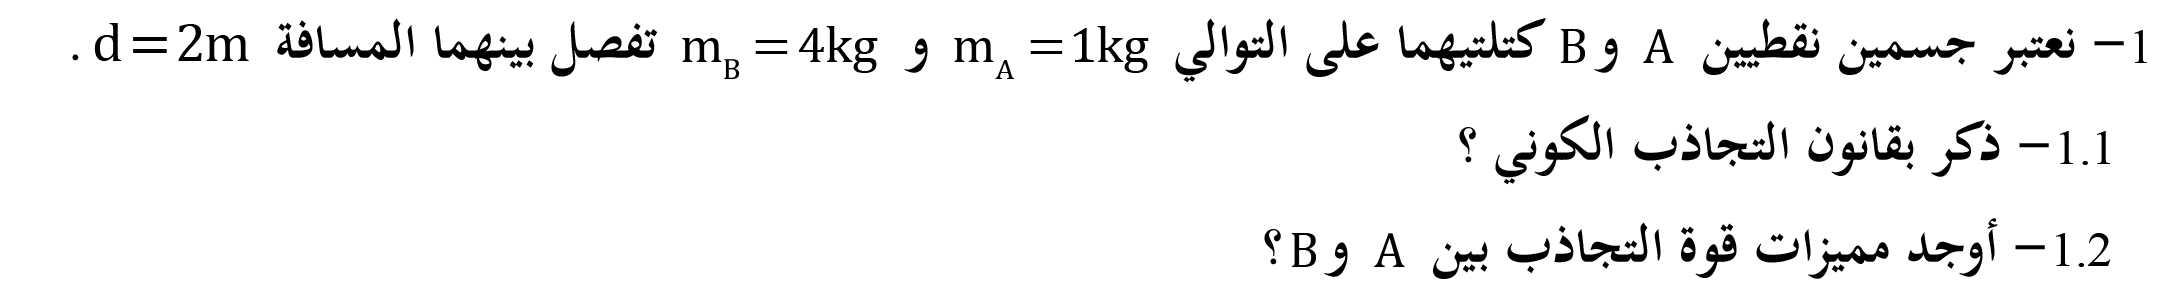
\includegraphics[width=\linewidth]{images/Tc/p1/e12_1.png}
					
\includegraphics[width=\linewidth]{images/Tc/p1/e12_2.png}
					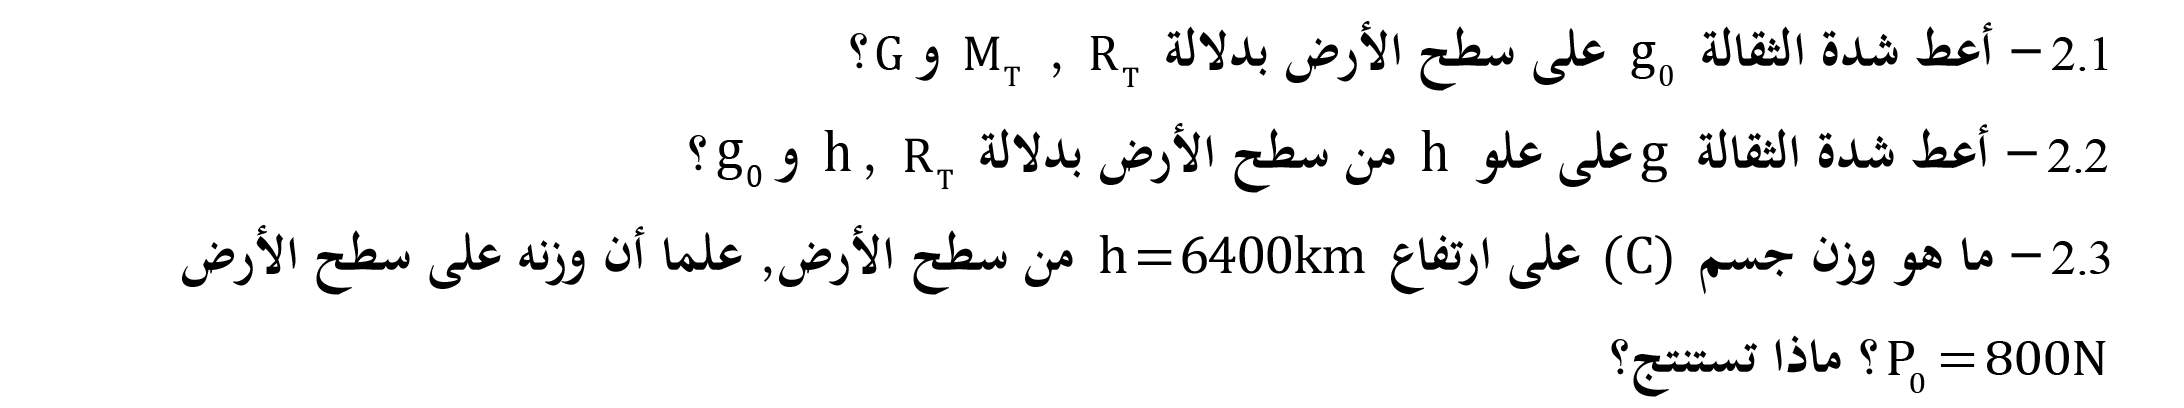
\includegraphics[width=\linewidth]{images/Tc/p1/e12_3.png}
					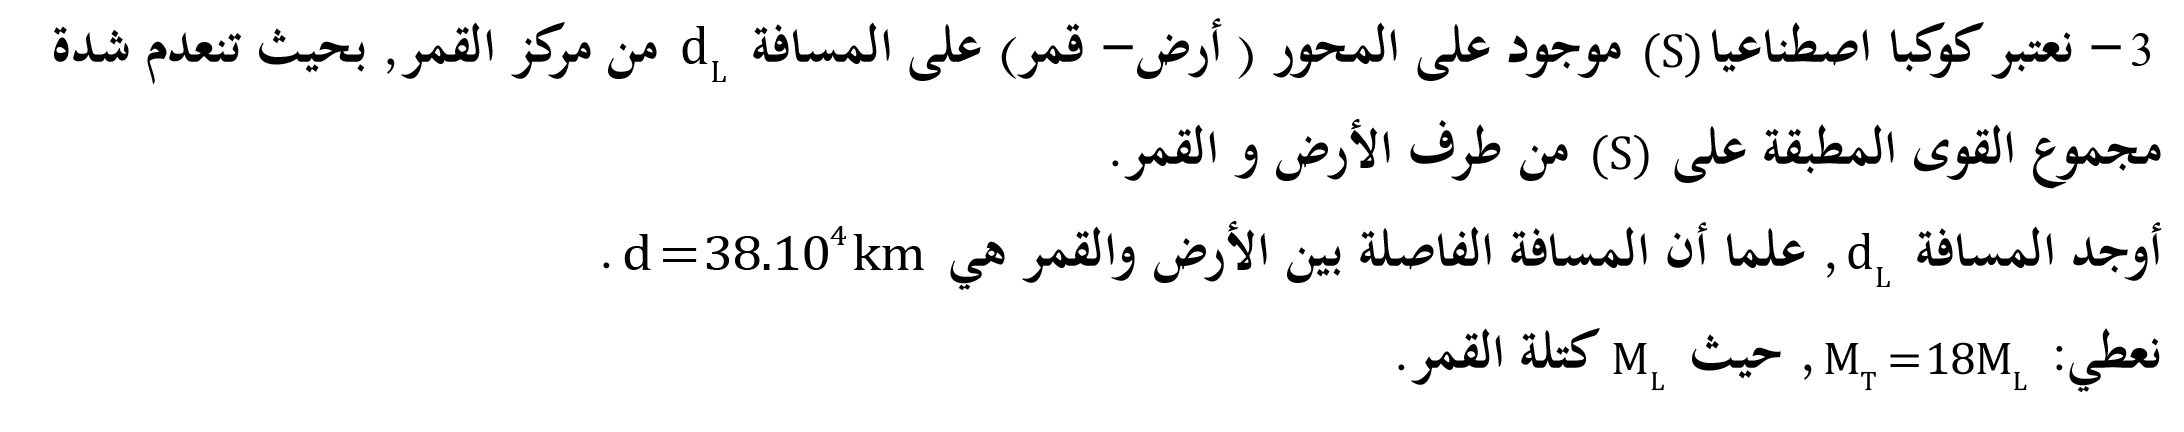
\includegraphics[width=\linewidth]{images/Tc/p1/e12_4.png}
					\end{exercice}%=== source ===%
  %Exercice 23
\begin{exercice}{}/
					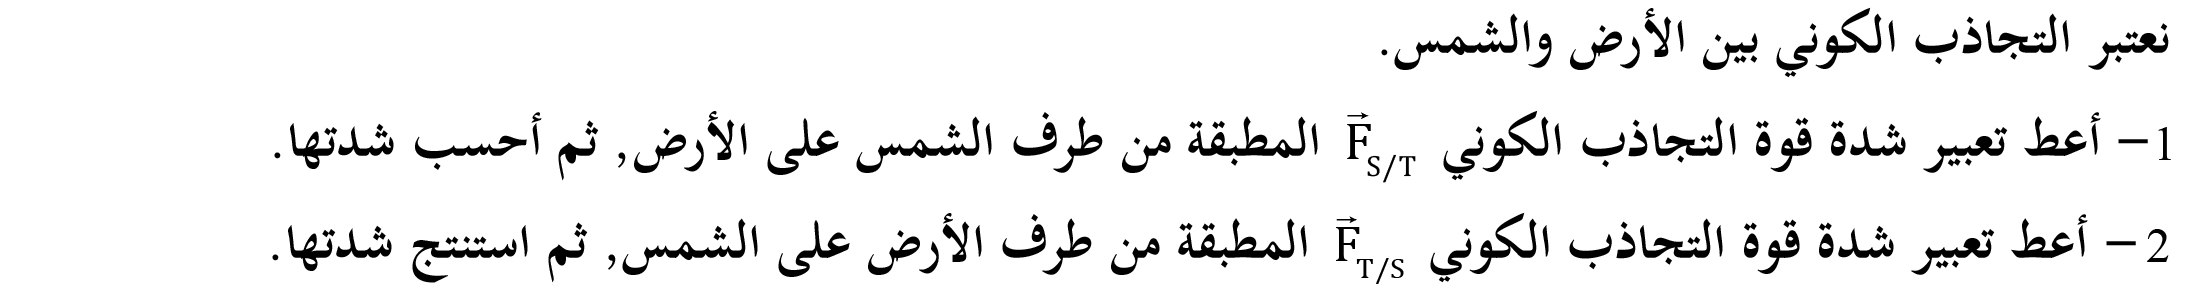
\includegraphics[width=\linewidth]{images/Tc/p1/e13_1.png}
					
\includegraphics[width=\linewidth]{images/Tc/p1/e13_2.png}
					\end{exercice}%=== source ===%  
  %Exercice 24
\begin{exercice}{}/
					
\includegraphics[width=\linewidth]{images/Tc/p1/e14_1.png}
					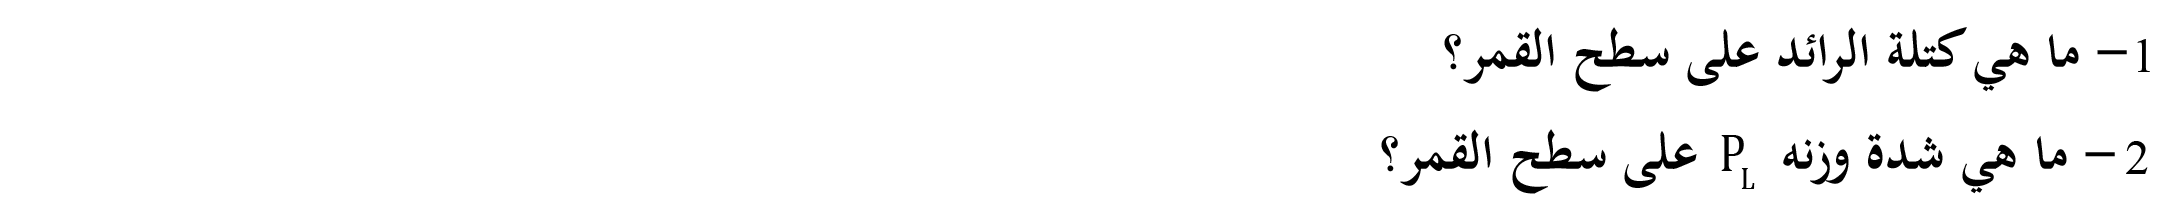
\includegraphics[width=\linewidth]{images/Tc/p1/e14_2.png}
					\end{exercice}%=== source ===%  
  %Exercice 25
\begin{exercice}{}/
					
\includegraphics[width=\linewidth]{images/Tc/p1/e16_1.png}
					
\includegraphics[width=\linewidth]{images/Tc/p1/e16_2.png}
					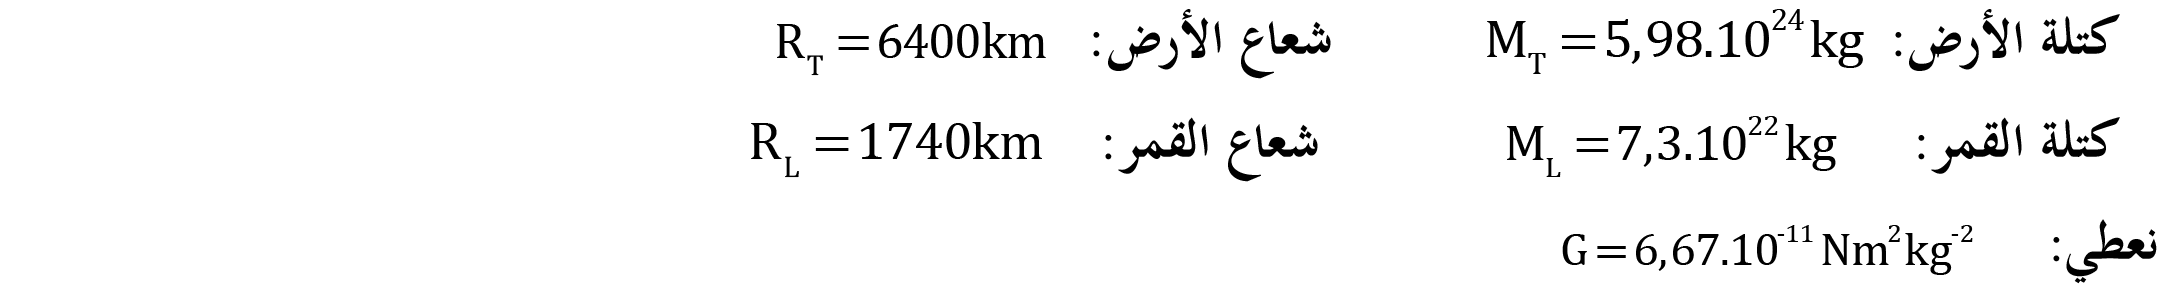
\includegraphics[width=\linewidth]{images/Tc/p1/e16_3.png}
					\end{exercice}%=== source ===% 
  
\end{document}